\documentclass[a4paper,11pt]{book}

% Import package settings.
\usepackage{syntonly}
% \syntaxonly

% \usepackage{indentfirst}
% \setlength{\parindent}{2em}
% -or-
\usepackage[parfill]{parskip}

\usepackage{hyperref}

% style=ieee-alphabetic
\usepackage[backend=biber,style=ieee]{biblatex}
\addbibresource{biblatex.bib}

\usepackage{graphicx}
\graphicspath{{./figs/}{./}}
\usepackage{subcaption}

\usepackage{lscape} % PDF page contents landscape
\usepackage{pdflscape} % PDF page landscape

\usepackage[toc,page]{appendix}

\usepackage{amsmath}
\usepackage{amssymb}
\usepackage{mathtools}

\usepackage{multicol}

\usepackage{pgfplotstable}
\usepackage{booktabs}

\usepackage[round-mode=places,round-precision=3]{siunitx}

\usepackage{pgfplots}
\pgfplotsset{compat=newest} % Allows to place the legend below plot
\usepgfplotslibrary{units} % Allows to enter the units nicely

% draw math injection
\usepackage[all]{xypic}

% draw diagonally divided table cell
% \usepackage{slashbox} % ancient and deprecated
\usepackage{diagbox}

% add underline to text
\usepackage{ulem}

% chemical equations
\usepackage[version=4]{mhchem}

% insert PDF page
\usepackage{pdfpages}

% allow \verb within the argument of another macro
\usepackage{cprotect}

%%% Local Variables:
%%% mode: latex
%%% TeX-master: "main"
%%% End:

\usepackage{fontspec}

% Western fonts by 'fontspec':
\setmainfont{Tinos}[ % search font by filename
  Path = /opt/fonts/core/Tinos/,
  Extension = .ttf,
  UprightFont = *-Regular,
  BoldFont = *-Bold,
  ItalicFont = *-Italic,
  BoldItalicFont = *-BoldItalic
]
\setsansfont{NotoSans}[ % search by 'postscriptname'
  BoldFont = NotoSans-Bold,
  ItalicFont = NotoSans-Italic,
  BoldItalicFont = NotoSans-BoldItalic  
]
\setmonofont{migu-1m-regular}[
  BoldFont = migu-1m-bold
]

% Chinese fonts by 'fontspec':
%
% \setmainfont{Adobe Song Std}
% \setsansfont{Noto Sans S Chinese}
% \setmonofont{Adobe Fangsong Std}
% \XeTeXlinebreaklocale "zh"
% \XeTeXlinebreakskip = 0pt plus 1pt minus 0.1pt
% \usepackage[top=1in,bottom=1in,left=1.2in,right=1in]{geometry}


% Chinese fonts by 'xeCJK':
\usepackage[boldfont]{xeCJK}
\setCJKmainfont{Adobe Song Std}[ % search by 'family'
BoldFont = NotoSansHans-Bold % search by 'postscriptname'
                             % because 'NotoSansHans' family has
                             % multiple variants.
]
\setCJKsansfont{NotoSansHans-DemiLight}[
  BoldFont = NotoSansHans-Bold
]
\setCJKmonofont{AdobeFangsongStd-Regular}[
  Path = /opt/fonts/core/AdobeStd/,
  Extension = .otf
]

% set new font family
\setCJKfamilyfont{zhyahei}{msyh}[ % search font by filename
  Path = fonts/,
  Extension = .ttf,
  BoldFont = {*bd}
]
% create font family command alias
\NewDocumentCommand{\yahei}{}{\CJKfamily{zhyahei}}


% Chinese fonts by 'xeCJK' from 'CTeX':
%
% \usepackage[UTF8,heading=true]{ctex}

% \setcjkmainfont{Adobe Song Std} % search by `family'
% \setCJKsansfont{NotoSansHans-DemiLight}[
%   BoldFont = NotoSansHans-Bold
% ]
% \setCJKmonofont{Adobe Fangsong Std}

%%% Local Variables:
%%% mode: latex
%%% TeX-master: "main"
%%% End:

\input{listings}

% Tell `include' to only include these sources in the body.
\includeonly{preface,resources,chinese,tutorial,combinatorics,tree,stack,c,cpp,sequenceOfNumber,brainteaser,aat,chemistry,appendices,postscript}


\begin{document}

\frontmatter{}

\title{Miscellanies}
\author{西二闲画生\\
  Department of Life,\\
  Zhonghua Uni.,\\
  WH, China\\
  \emph{zhu@riseup.net}}
\date{\today}
\maketitle


\chapter{Preface}
\label{cha:preface}

\LaTeX{} typesets text as \textit{What You See Is What You Type}
compared with \textit{What You See Is What You Get}. It gives
finer control over text layout with a host of commands and
add-ons. This book firstly demonstrates how \LaTeX{} supports
Chinese typesetting and then moves on to syntax. A bit of ACTeX
with Emacs configuration and key bindings are dicussed as
well. Gradually, topics from different disciplines (i.e. math and
language) are introduced in separate parts.

Priorly, I just planned to learn \LaTeX{} through trial and
error. As it progressed, I found \LaTeX{} an awesome typesetting
tool, creating beautiful text output. Hence, I decided to make
it a book containing different parts, covering formal subjects
like math, physics, etc. Ultimately, I want to maintain a
centralized offline jottings which can be testified by the book
title \textit{Miscellanies}.

%%% Local Variables:
%%% mode: latex
%%% TeX-master: "main"
%%% End:


\setcounter{tocdepth}{3} % Show subsubsections
\tableofcontents{}

\mainmatter{}

\part{\LaTeX{}}
\chapter{\LaTeX{} Resources}
\label{cha:latex-resources}

\section{Find References}
\label{sec:find-references}

In part \ref{cha:inputChinese} on page
\pageref{cha:inputChinese}, we have a simple clarification on
how to insert Chinese characters in English articles. We will
focus on \LaTeX{} itself in this part.

Please find more appropriate at
\href{https://ctan.org/topic/tut-latex?lang=en}{\LaTeX{}
  ctan}. Also, please find anwsers at
\cite{stackexchange}. You'd better go through the tutorial series
\cite{tutorial}. My personal webiste \cite{zhstar} might give some
ideas.

\section{AUCTeX}
\label{sec:auctex}

\subsection{Inserting}
\label{sec:inserting}

\begin{table}[tbp]
  \centering
  \begin{tabular}{|l|l|}
    \hline{}
    Binding & Function \\ \hline \hline{}
    \verb|C-c C-e| & insert environment \\ \hline{}
    \verb|C-c C-s| & insert section \\ \hline{}
    \verb|C-c C-m| & macro (command) \\ \hline{}
    \verb|M-return| & another item \\ \hline{}
    \verb|C-c C-c| & compile \LaTeX{} \\ \hline{}
    \verb|C-c C-v| & preview output \\ \hline{}
    \verb|C-c =| & show document layout by RefTeX \\ \hline{}
    \verb|C-c C-o C-b| & fold the buffer \\ \hline{}
    \verb|C-c C-o b| & unfold the buffer \\ \hline{}
    \verb|C-c C-r| & compile selected region \\ \hline{}
    \verb|C-c C-b| & compile current buffer \\ \hline
  \end{tabular}
  \caption{AUCTeX Bindings}
  \label{tab:auctex-bindings}
\end{table}

Have a look at
\href{https://github.com/bigclean/blogs/blob/master/emacs/auctex.mkd}{\LaTeX{}}

\subsection{\LaTeX{} Sources Formating}
\label{sec:code-formating}

Use \verb|C-c C-q C-s| to format \LaTeX{} \textit{section}
code. \verb|C-c C-q C-p| is to format \textit{paragraph} text.

\subsection{Font Specifiers}
\label{sec:font-specifiers}

Use \verb|C-c C-f C-i| to insert \textit{italic} text. Smililary,
Use \verb|C-c C-f C-b| to insert \textit{bold} text. Read more at \href{https://www.gnu.org/software/auctex/manual/auctex/Font-Specifiers.html}{Insert Font Spcecifiers}.

\begin{center}
  \begin{tabular}{|l|l|}
    \hline{}
    C-c C-f C-i	& italic \\ \hline{}
    C-c C-f C-b & bold \\ \hline{}
    C-c C-f C-e & emphasize \\ \hline{}
    C-c C-f C-s & slight italic \\ \hline{}
    C-c C-f C-r & roman \\ \hline{}
    C-c C-f C-f & sans \\ \hline{}
    C-c C-f C-d & delete font formating \\ \hline
  \end{tabular}
\end{center}

%%% Local Variables:
%%% mode: latex
%%% TeX-master: "main"
%%% End:

\chapter{汉语}
\label{cha:inputChinese}

对字体的引用要注意,如果一个字体族 family 有多个变种 \footnote{如
  regular, bold, italic 等。},请引用字体的 postscriptname.

默认情况下,\LaTeX{} 会把文档里用到的字体子集内嵌到生成的 PDF 里,
可以通过命令行 \textit{pdffonts filename.pdf} 查询,结果
如 \ref{cha:long-code-line} 所示。

此例说明,对应文档内嵌了七个字体子集。\LaTeX{} 文档通常只会用到字
体文件的部分 code point,所以只需要内嵌使用到的部分即可。每个字体
的前面都有一串无规则字母,代表对应字体文件被内嵌的子集。还有一列叫
sub 也说明是否是子集。

\section{CJK 包}

在英文文档里插入少量中文

\subsection{CJK 和 CJK* 环境}
在英文文档里用 CJK 包的 CJK 或 CJK* 环境插入少量汉字。后者会忽略汉
字后面的空格,推荐使用。

\subsection{字体}
bsmi~字体可能没有,尝试换一个如~gkai, ~gbsn~等。

\section{xeCJK 更好}
xeCJK 在处理细节上更好,关键是可方便设置中英文字体。用 xeCJK 则不需
要特殊环境包裹汉字,只需在``导言区''设置好中英文字体即可。

xeCJK 的 indentfirst 选项:
\begin{center}
  \verb|\usepackage[indentfirst]{xeCJK}|
\end{center}
已过时,推荐直接用 indentfirst 宏包:
\begin{center}
  \verb|\usepackage{indentfirst}|
\end{center}

\section{fontspec 和 ctex}
\label{sec:fontspec-ctex}

还有 \textit{fontspec} 和 \textit{ctex} 包可以实现中文输入,更多详
情请看 \href{https://www.zhstar.win/2015/02/05/LaTeX/}{\LaTeX{}
  post}.

\begin{itemize}
\item \verb|fontspec| sets western or Chinese fonts (i.e. main, sans, serif, bold, italic, and bolditalic).
\item \verb|CJK| sets Chinese, Japanese, and Korean fonts, punctuation etc. for TeX engine.
\item \verb|xeCJK| similar tof \verb|CJK| but for XeTeX engine.
\item \verb|CTeX| sets \verb|CJK/xeCJK| document layout.
\end{itemize}

\section{中英文空格}
我们想要的效果是英文字符前后自动加上空格。xeCJK 则会自动处理,但是
效果不是非常好。

CJK 会忽略 \TeX{} 源码里的空格。用 CJK 宏集里的 CJKspace 包,源码里
英文后空格会保留,中文后空格依然被 CJK* 压缩。还有一个方法是在需要空
格的地方用 tilde $\sim$.

\section{行首缩进}

中文习惯每段行首缩进两个汉字。英文有两种缩进格式。默认是每小节的第
一段缩进,后面的段不缩进,段间没有空行。另一种是不缩进,每段间留有
空行。

本文档只插入少量中文作例子,固保留英文默认缩进方式。如要换成中文缩
进,则用 indentfirst 包,使每节第一段也缩进,如下:
\begin{center}
  \begin{tabular}{l}
    \verb|\usepackage{indentfirst}| \\
    \verb|\setlength{\parindent}{2em}|
  \end{tabular}
\end{center}
如若换成英文第二种缩进,则
用\href{https://tex.stackexchange.com/a/40432}{parskip} 包,skip 表
示相临两段之间的间隙大小:
\begin{center}
  \begin{tabular}{l}
    \verb|\usepackage[parfill]{parskip}|
  \end{tabular}
\end{center}
也可用相对应的命令实现:
\begin{center}
  \begin{tabular}{l}
    \verb|\setlength{\parindent}{0pt}| \\
    \verb|\setlength{\parskip}{1ex plus 0.5ex minus 0.2ex}|
  \end{tabular}
\end{center}

\section{局部字体命令}

前面提到的方法都是全局生效,有没有类似 \verb|\emph{}| 和
\verb|\textit{}| 这种监时改中文字体的方法呢?

在 \textit{xecjk.tex} 中有如下代码:

\begin{lstlisting}[language=TeX,caption={New font family},label={lst:new-font-family}]
% set new font family
\setCJKfamilyfont{zhyahei}{msyh}[
  Path = fonts/,
  Extension = .ttf,
  BoldFont = {*bd}
]

% create font family command alias
\NewDocumentCommand{\yahei}{}{\CJKfamily{zhyahei}}
\end{lstlisting}

根据需求定义一个新的字体族 family 名 \textit{zhyahei},新字体族的
引用方法是:

\begin{lstlisting}[language=TeX,caption={Inline Chinese fonts},label={lst:inline-chn-fonts}]
{\CJKfamily{zhyahei}{这里输中文}}
% -or-
{\CJKfamily{zhyahei}这里输中文}
\end{lstlisting}

为了方便,我们还定义一个新 NewDocumentCommand 命令,便于快速引
用。\verb|{\yahei{这是新定义的雅黑字体样例。}}| 的效果
如:{\yahei{这是新定义的雅黑字体样例。}}

特别注总,命令要放在一个 group 里,即用 \verb|{}| 围起来,否则从当
前位置起,所有中文字体都改了。实际,fontspec 提供类似功能,具体请参
考 fontspec 文档。如:

\begin{center}
  \verb|\fontspec{⟨font name⟩}[⟨fontfeatures⟩]| 和 \verb|\newfontfamily|
\end{center}


%%% Local Variables:
%%% mode: latex
%%% TeX-master: "main"
%%% End:

\chapter{\LaTeX{} Tutorial}
\label{cha:latex-tutorial}

\section{\TeX{} Units}
\label{sec:tex-units}

\begin{figure}[h]
  \centering
  \includegraphics[width=.5\textwidth]{units}
  \caption{\TeX{} Units}
  \label{fig:tex-units}
\end{figure}

\section{Special characters}
\label{sec:special-characters}

The following 10 characters has special meanings in
\LaTeX{}.

\begin{center}
  \verb|& % $ # _ { } ~ ^ \|
\end{center}

Outside \textit{verb}, the first 7 should escaped by
\textit{backslash}. Of the last three, we use \LaTeX{} macros,
namely \verb|\textasciitilde|, \verb|\textasciicircum| and
\verb|\textbackslash|.

\begin{lstlisting}[language=TeX,caption={Special Characters},label={lst:special-characters}]
\& \% \$ \# \_ \{ \} \textasciitilde{} \textasciicircum{} \textbackslash{}
\end{lstlisting}

Specially, \LaTeX{} uses tilde \textasciitilde{} as a non-breaking space. You
would usually use non-breaking spaces for punctuation marks in
some languages, for units and currencies, for initials, etc.

\section{verbatim and verb}
\label{sec:verbatim-verb}

When to show raw text without \LaTeX{} command being executed, use
\textit{verbatim} environment or \textit{verb} command. Both have
an asterisk alternative like \verb|\begin{verbatim*}| and
  \verb|\verb*|. With extra *, \LaTeX{} will typewrite space as
\texttt{␣}.

You can't use \texttt{\textbackslash{}verb} in other command's
parameters. For example, this is not allowed:

\begin{lstlisting}[language=TeX,caption={Illegal verb}]
\href{https://tex.stackexchange.com/a/23653}{When should we use
  \verb|\begin{center}| instead of \verb|\centering|?}
\end{lstlisting}

Instead, we use
\href{https://tex.stackexchange.com/q/2790}{\texttt{\textbackslash{}texttt}}
and escape special characters \footnote{For instance, backslash
and \{.} like:

\begin{lstlisting}[language=TeX,caption={texttt}]
\href{https://tex.stackexchange.com/a/23653}{When should we use
\texttt{\textbackslash{}begin\{center\}} instead of \texttt{\textbackslash{}centering}?}
\end{lstlisting}

\section{item list}
\label{sec:item-list}

Using lists is quite straightforward and does not require you to
add any additional packages. For unordered list, \LaTeX{} provides
the \textit{itemize} environment and for ordered list there is the
\textit{emunerate} environment. With both environments, elements
should be declared beginning with \verb|\item| command. We can use
\verb|M-Enter| binding to insert this command automatically.

Take a look at unordered list\ref{lst:itemize-unordered-list}:

\begin{minipage}{.4\linewidth}
\begin{lstlisting}[label={lst:itemize-unordered-list},linewidth=.7\textwidth]
\begin{itemize}
\item One
\item HKUST
\item HUST
\end{itemize}
\end{lstlisting}  
\end{minipage}
\hfill
\framebox{
\begin{minipage}{0.4\linewidth}
  \begin{itemize}
  \item One
  \item HUST
  \item HKUST
  \end{itemize}
\end{minipage}
}

Here is an ordered list \ref{lst:enumerate-ordered-list}:

\begin{minipage}{.4\linewidth}
  \begin{enumerate}
  \item Jim
  \item Gray
    \begin{itemize}
    \item This is a
    \item nested unordered
    \item list within ordered list
    \end{itemize}
  \item Who are you?
  \end{enumerate}
\end{minipage}
\hfill{}
\begin{minipage}{.4\linewidth}
\begin{lstlisting}[label={lst:enumerate-ordered-list}]
\begin{enumerate}
\item Jim
\item Gray
  \begin{itemize}
  \item This is a
  \item nested unordered
  \item list within ordered list
  \end{itemize}
\item Who are you?
\end{enumerate}
\end{lstlisting}
\end{minipage}

\section{Code listings}
\label{sec:code-listings}

Although \textit{verb} and \textit{verbatim} enclose raw text,
they don't highlight source code like C, Java etc. This is where
\textit{listings} package come into
\href{https://en.wikibooks.org/wiki/LaTeX/Source_Code_Listings}{usage}.

To insert a code block, use \textit{lstlisting} environment like

\begin{center}
  \verb|\begin{lstlisting}[language=bash,caption={Bash},frame=single]|
\end{center}

Here is an example:

\begin{lstlisting}[language=bash,caption={Bash},frame=single]
#!/bin/bash
echo 'Hello, world!'
\end{lstlisting}

Furthermore,
\begin{lstlisting}[language=TeX,caption={Include code file},breaklines]
\lstinputlisting[language=C,frame=tb,basicstyle=\scriptsize\ttfamily]{helloworld.c}
\end{lstlisting}
command includes code source file:
\lstinputlisting[language=C,frame=single,
caption={C98}]{helloworld.c} This is useful when the code needs
updating frequently.

To prevent \textit{lstlisting} from breaking pages, we should wrap
it within \textit{minipage} environment as \ref{lst:table-floating}.

Sometimes, code line is too long to fit page width, leaving
tailing part out of page. We could modify \textit{basicstyle} to
one of \textit{footnotesize}, \textit{scriptsize} and
\textit{tiny}. Check long text line example
\ref{cha:long-code-line}. For more options, read
\href{https://tug.org/texinfohtml/latex2e.html#Font-sizes}{Font
  Size} and \href{https://tex.stackexchange.com/q/24599}{font size
  and point (pt) relation}.

{\LARGE This is LARGE text} {\Huge while this is Huge}.

\section{Straight Quotes}
\label{sec:straight-quotes}

By default, \textit{listings} typesets both single and double as
\textit{back curve ones}.

We should import \textit{textcomp} package and \textit{fontenc}
package with \href{https://tex.stackexchange.com/a/677}{T1}
option. Then, enable \textit{upquote=true} for code block. Read
more at \href{https://tex.stackexchange.com/q/166790}{How can I
  get straight double quotes in listings?}

This method, however, is discouraged as \textit{fontenc} would
override the whole document \LaTeX{} font settings. The underlying
cause is \textit{serif (roman)} font. Default roman fonts does not
provide straight quotes. We should tell \textit{listings} to use
\textit{monospace} font instead by

\begin{center}
  \verb|\lstset{basicstyle=\ttfamily}|
\end{center}

Read more at
\href{https://tex.stackexchange.com/q/144396}{Consolas: Straight
  Quotes}.

\section{floating}
\label{sec:floating}

\subsection{Figure}
\label{sec:figure}

First, we import \textit{graphicx} package and then set
\textit{graphicspath} in preamble part:
\begin{lstlisting}[language=TeX,caption={graphicx}]
\usepackage{graphicx}
\graphicspath{{figs/}{./}}
\end{lstlisting}

\textit{graphicx} accepts EPS, PDF, PNG or JPEG
formats. \textit{graphicspath} defines a list of directories
relative to that of \textit{master.tex}. By this means, we can
access images anywhere without restriction like
\verb|\graphicspath{{../../img/}}|. The trailing slash cannot be
omitted.

Then, we use command \textit{includegraphics} like

\begin{center}
  \verb|\includegraphics[width=.5\textwidth,scale=0.1]{myimg}|
\end{center}

Notice that we do not write figure file extension. Here is the
output:
\begin{center}
  \includegraphics[width=.5\textwidth,scale=0.1]{leg}
\end{center}

With bare \textit{includegraphics}, if remaining space within current
page does not hold the figure, \LaTeX{} would start a new page
instead, leaving current page partially emtpy. The method is to
wrap it with \textit{figure} environment:

\begin{minipage}[top]{1.0\linewidth}
\begin{lstlisting}[language=TeX,caption={Figure Floating}]
\begin{figure}[tbp]
  \centering
  \includegraphics[width=\textwidth]{Boobs}
  \caption{Boobs}
  \label{fig:Boobs}
\end{figure}
\end{lstlisting}  
\end{minipage}

We call this technique as \textit{floating}. Apart from
\textit{placement specifier} benefits, we can define
\textit{label} and \textit{caption} within \textit{floating}
environment. Note that \verb|\label{}| command must come
\textbf{after} \verb|\caption{}| command since the reference
number is generated by \verb|\caption{}|. For details, refer to
\href{https://tex.stackexchange.com/a/32326}{Why does an
  environment's label have to appear after the caption?}.

The \verb|tbp| \footnote{\textit{tbp} is the default
  \textit{placement specifier}. We could set it to
  \textit{!htbp}.} specifies position of floating environment.

\begin{figure}[h]
  \centering
  \includegraphics[width=.5\textwidth]{floating}
  \caption{Floating Placement Specifiers}
  \label{fig:placement-specifiers}
\end{figure}

Here is a nice boobs example \ref{fig:boobs}:

\begin{figure}[!htbp]
  \centering
  \includegraphics[scale=.3]{boobs}
  \caption{boobs}
  \label{fig:boobs}
\end{figure}

Sometimes, it's necessary to put figures side by side for clear
comparasion. We use \textit{subfigure} within \textit{figure} like
\ref{fig:three-girsl}. Please be noted that we add non-breakable
symbol \textasciitilde{} between \textit{subfigure} to leave
some space between figures.

\begin{figure}[tbp]
  \centering
  \begin{subfigure}[tbp]{0.3\linewidth}
    \includegraphics[width=\linewidth]{sub1}
    \caption{Girl A}
  \end{subfigure}
  ~
  \begin{subfigure}[tbp]{0.3\linewidth}
    \includegraphics[width=\linewidth]{sub2}
    \caption{Girl B}
  \end{subfigure}
  ~
  \begin{subfigure}[tbp]{0.3\linewidth}
    \includegraphics[width=\linewidth]{sub3}
    \caption{Girl C}
  \end{subfigure}
  \caption{Three Girls}
  \label{fig:three-girsl}
\end{figure}

\subsection{Table}
\label{sec:table}

Similarly, we can wrap \textit{tabular} within \textit{table}
environment to \textit{float} table \ref{tab:auctex-bindings} like
\ref{lst:table-floating}.

\begin{minipage}[top]{1.0\linewidth}
\begin{lstlisting}[language=TeX,caption={Table Floating},label={lst:table-floating}]
\begin{table}[!htbp]
  \centering
  \begin{tabular}{|l|r|}
    \hline{}
    Binding & Function \\ \hline \hline{}
    \verb|C-c C-e| & insert environment \\ \hline{}
    \verb|C-c C-s| & insert section \\ \hline{}
    \verb|C-c C-m| & macro (command) \\ \hline{}
    \verb|M-return| & another item \\ \hline{}
    \verb|C-c C-c| & compile \LaTeX{} \\ \hline{}
    \verb|C-c C-v| & preview output \\ \hline{}
    \verb|C-c =| & show document layout by RefTeX \\ \hline{}
    \verb|C-c C-o C-b| & fold the buffer \\ \hline{}
    \verb|C-c C-o b| & unfold the buffer \\ \hline
  \end{tabular}
  \caption{AUCTeX Bindings}
  \label{tab:auctex-bindings}
\end{table}
\end{lstlisting}
\end{minipage}

In \textit{tabular} environment, we align column texts as
\textit{\textbf{l}eft}, \textit{\textbf{c}enter} and
\textit{\textbf{r}ight}. What about decimal number cell? Idealy,
we want to align numbers at dot, where package \textit{siunitx}
plays a role by \textbf{S} \ref{tab:number-alignment-at-dot}
alignment specifier.

\begin{lstlisting}[language=TeX,caption={Decimal Alignment},label={lst:decimal-alignment}]
\usepackage[round-mode=places,round-precision=3]{siunitx}
\end{lstlisting}

To make prettier table, we use package \textit{booktabs} which
provides \textit{toprule}, \textit{midrule} and
\textit{bottomrule} to override \footnote{It is not replace!} dull \textit{hline}.

\begin{table}[tbp]
  \centering
  \begin{tabular}{l|S|r}
    \toprule{}
    \textbf{List 1} & \textbf{Decimal 2} & \textbf{Letter 3} \\
    $\alpha$ & $\beta$ & $\gamma{}$ \\
    \midrule{}
    1 & 1385.1 & a \\
    2 & 3.0674 & b \\
    3 & 87.369 & c \\
    \bottomrule
  \end{tabular}
  \caption{Number Alignment at Dot}
  \label{tab:number-alignment-at-dot}
\end{table}

To make more complex tables, we can use package \textit{multirow}
and \textit{multirow} and \textit{multicolumn} environment
respectivelly.

When typesetting large tables, it is tedious and error-prone which
could be avoided by \textit{pgfplotstable} package that generate
tables from external \textit{.csv} file. Programs such as Excel,
OpenOffice Calc or even emacs org-mode can export data sheets as
\textit{.csv} files. The \textit{pgfplotstable template}
\ref{sec:pgfplotstable-template} generate table
\ref{table-automation-from-csv}.

\begin{table}[tbp]
  \centering{}
  \pgfplotstabletypeset[
    multicolumn names,
    col sep=comma,
    display columns/0/.style={
      column name=$Ampere$,
      column type={S},string type
    },
    display columns/1/.style={
      column name=$Voltage$,
      column type={S},string type
    },
    display columns/2/.style={
      column name=$Energy$,
      column type={S},string type
    },
    every head row/.style={
      before row={\toprule},
      after row={
        \si{\ampere} & \si{\volt} & \si{\joule} \\
        \midrule
      }
    },
    every last row/.style={
      after row=\bottomrule
    },
  ]{pgfplotstable.csv}
  \caption{Table automation from .csv file.}
  \label{table-automation-from-csv}
\end{table}

\subsection{Plot}
\label{sec:plot}

The \textit{pgfplots} package is a powerful tool, based on
\textit{tikz} package, dedicated to create scientific
graphs. Similar to \textit{pgfplotstable}, \textit{pgfplots} can
read date from \textit{.csv} file.

Since \textit{pgfplots} is based on \textit{tikz}, the
\textit{axis} environment should be enclosed within
\textit{tikzpicture} environment. Template
\ref{lst:pgfplots-template} generates plot
\ref{fig:pgfplots-by-table-csv-file}.

\begin{figure}[!ht]
  \centering
  \begin{tikzpicture}
    \begin{axis}[
      width = \linewidth, % Scale the plot to \linewidth
      grid = major, grid style = dashed,
      xlabel = Voltage $U$, ylabel = Currency $I$, % Set the labels
      x unit = \si{\volt}, y unit = \si{\ampere}, % Set the respective units
      % axis lines = left % only display the left and bottom axes
      legend style = { at = {(0.5,-0.2)}, anchor = north }, % Put the legend below the plot
      x tick label style = { rotate = 90, anchor = east } % Display labels sideways
      ]
      % add a plot from table; you select the columns by using the
      % actual column header name in the .csv file
      \addplot
      table[x=value 1,y=value 2,col sep=comma]{pgfplots.csv};
      \legend{$U$ - $I$}
      % add another plot
      \addplot
      {x^2 - 2*x + 1}; % add a tailing semicolon
      \addlegendentry{$x^2 - 2x + 1$} % use addlegendentry instead of legend
    \end{axis}
  \end{tikzpicture}
  \caption{pgfplots by table csv file}
  \label{fig:pgfplots-by-table-csv-file}
\end{figure}

\textit{addplot} plots 2D figure, for 3D, we use \textit{addplot3}
\ref{fig:pgfplots-3d}.

\begin{figure}[tbp]
  \centering
  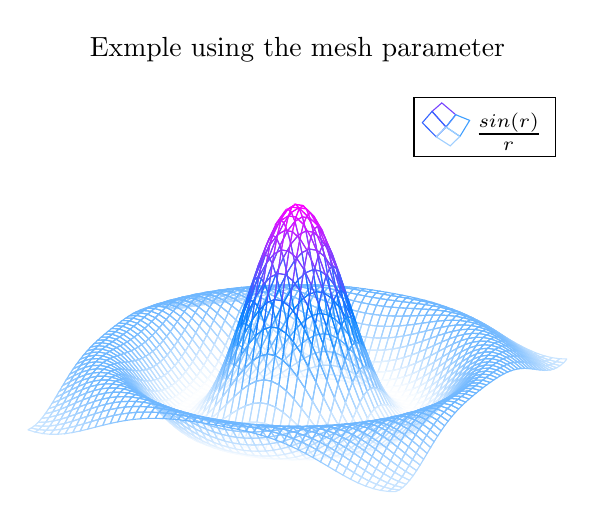
\begin{tikzpicture}
    \begin{axis}[
      title=Exmple using the mesh parameter,
      hide axis,
      colormap/cool,
      ]
      \addplot3[ mesh, samples=50, domain=-8:8, ]
      {sin(deg(sqrt(x^2+y^2)))/sqrt(x^2+y^2)};
      \addlegendentry{$\frac{sin(r)}{r}$}
      \end{axis}
  \end{tikzpicture}  
  \caption{pgfplots 3D}
  \label{fig:pgfplots-3d}
\end{figure}

Besides \textit{pgfplotstable} and \textit{pgfplots}, we could
aslo use \textit{tgiz} package or \textit{circuitkiz} to
\verb|\draw| pictures from within your LaTeX document.

\section{center and centering}
\label{sec:center-centering}

The main difference between \textit{center} environment and
\textit{centering} command is the former leave vertical space
before and after it while the later would not.

We usually use \verb|\centering{}| command within a group by curly
braces, figure, table, or
\verb|\begingroup \centering ... \endgroup|
\ref{lst:centering-within-braces}.

\begin{minipage}{1.0\linewidth}
\begin{lstlisting}[language=TeX,caption={centering within braces},label={lst:centering-within-braces}]
{\centering{centering require line break by \par, emtpy line or \\
before closing the group, otherwise text following the group wound
be centered either.}\\
}
\end{lstlisting}  
\end{minipage}

{\centering{centering require line break by \verb|\par|, emtpy
    line or \verb|\\| before closing the group, otherwise text
    following the group wound be centered either.}

} This line is not centered! Check
\href{https://tex.stackexchange.com/a/23653}{When should we use
  \texttt{\textbackslash{}begin\{center\}} instead of
  \texttt{\textbackslash{}centering}?} and
\href{http://texblog.net/latex-archive/floats/center-centering/}{center
  vs. centering}

\section{Math Equations}
\label{sec:math-equations}

To insert simple inline equation, we wrap it by \$ like
\verb|$c^2=a^2+b^2$|: $c^2=a^2+b^2$.

For tall or deep inline math expressions or sub expressions, we
can enclose them by \verb|\smash| command. This makes \LaTeX{}
ignore the height of these expressions. This keeps the line
spacing even like: \smash{$d_{e_{e_p}}$} followed by
\smash{$h^{i^{g^h}}$}.

This is an example without \verb|\smash|. You will find line space
is much bigger. A $d_{e_{e_p}}$ expression followed by a
$h^{i^{g^h}}$ one.

If we want equaton occupy a whole line, then wrap it by double
\$\$ or single bracket \verb|\[\]|. The equation will be centered
automatically.

\begin{lstlisting}[language=TeX,caption={Equation in new line},label={lst:equation-in-new-line}]
$$(1+x)^n=\sum_{k=0}^n\binom{n}{k}x^k$$
\end{lstlisting}

This is the output:
$$(1+x)^n=\sum_{k=0}^n\binom{n}{k}x^k$$
Let's have another example:
$$A_1+A_{100}$$

After examing the example above, you are recommended to tune
AUCTeX \ref{sec:auctex} configuration a little bit. Enable math
mode manually by \verb|C-c ~| or globally into Emacs startup:

\begin{lstlisting}[language=Lisp,caption={\LaTeX{} Math Mode},label={lst:latex-math-mode}]
(add-hook 'LaTeX-mode-hook 'LaTeX-math-mode)
\end{lstlisting}

We just prepend \verb|`| and type your desired math symbol. AUCTeX
automatically completes it. If given a prefix argument \verb|C-u|,
the symbol will be surrounded by dollar signs. For example, if you
type \verb|C-u ` b|, AUCTex will typeset \verb|$\beta$|. Read
AUCTex manual
\href{https://www.gnu.org/software/auctex/manual/auctex/Mathematics.html}{Entering
  Mathematics} for more details.

The \$ method by \TeX{} does provide some basic mathematics
features, but it is limited. we should
\verb|\usepackage{amsmath}|. What is more, we can
\verb|\usepackage{amssymb}| to make math symbols look shiny.

A bit further, we usually want to label and number a equation so
that we can refer to it somewhere else. Futhermore, it is better
for a long equation to occupy a new line. To do this, enclose
equation with \textit{equation} environment like
\eqref{eq:einstein}. Einstein says

\begin{equation}
  \label{eq:einstein}
  E = mc^2
\end{equation}

In order that multiple equations align properly at
\textit{ampersand \&}, we use \textit{align} or \textit{align*}
instead.  \eqref{eq:eq-alignment}. Each single equation must be
separated by \textit{linebreak \\\\}. The version with asterisk
just removes equation numbers.

\begin{align}
  \label{eq:multi-eqs}
  E &= mc^2 \\
  F &= ma
\end{align}

We use \textit{aligned} environment to align induction or
substitution lines of a single equation. Also, \textit{aligned}
should be enclosed within an equation environment.

\[
  \begin{aligned}[t]
    \label{eq:eq-alignment}
    f(x) &= x^2 \\
    \frac{1}{x} &= g(x) \\
    F(x) &= \int^a_b \frac{1}{\sqrt[3]{x}}
  \end{aligned}
\]

Compared to \textit{aligned}, \textit{align} and \textit{align*}
introduce extra space between lines to make the output
cleaner. Therefore, irrespective of single equation or multiple
equations, we'd better use \textit{align} and/or\textit{align*}.

\textit{matrix} environment must be enclosed by equation marker \&
or \textit{equatioin} environment.

\begin{lstlisting}[language=TeX,caption={Matrix},label={lst:matrix-marker}]
$
\begin{matrix}
  1 & 0 \\
  0 & 1
\end{matrix}
$
\end{lstlisting}

Similary, matrix breaks line by \verb|\\| and \& separates
columns. Here is a \textit{bmatrix} example:

\begin{equation}
  \label{eq:nn-matrix}
  A_{m,n} =
  \begin{bmatrix}
    a_{1,1} & a_{1,2} & \cdots & a_{1,n} \\
    a_{2,1} & a_{2,2} & \cdots & a_{2,n} \\
    \vdots & \vdots & \ddots & \vdots \\
    a_{n,1} & a_{n,2} & \cdots & a_{n,n}
  \end{bmatrix}  
\end{equation}

Recall that \$\$ or \verb|\[\]| let an equation placed on a new
line without label. They are equivalent to the
\verb|\begin{equation*}| environment.

\section{Document Structure}
\label{sec:file-structure}

\section{Boxes}
\label{sec:boxes}

Everything in \LaTeX{} is embedded in boxes, from letter to words,
\textit{tabular} to \textit{includegraphics}. TeX builds pages by
gluing \footnote{Squeeze and/or Stretch} boxes together according
to the default \TeX{} rules, default \LaTeX{} rules, or document
commands.

\href{https://en.wikibooks.org/wiki/LaTeX/Boxes}{Box} is of
paramount importance to get the base of \LaTeX{} typestting. Boxes
are placed relative to other boxes, while visible elements are
placed relative to the boxes which contain them.

Let's have a look at letter box illustration \ref{fig:letter-box}.

\begin{figure}[!htbp]
  \centering
  \includegraphics[width=.5\textwidth]{letter_box}
  \caption{Letter Box}
  \label{fig:letter-box}
\end{figure}

\verb|\parbox| is a box to wrap text into lines and lines are
broken into pages.

\begin{lstlisting}[language=TeX,caption={parbox box},label={lst:parbox-box}]
\parbox[pos][height][contentpos]{width}{text}
\end{lstlisting}

\textit{width} is a forced parameter to define box
width\footnote{It is \textbf{not} text width.} This argument can
be relative value like \verb|.8\textwidth|, absolute value like
\verb|5ex|, or \LaTeX{} and \TeX{} macros like
\verb|\width|. Similarly, we set \textit{height} in the same way.

\textit{pos} selects which \textit{baseline} of text to align with
neighbouring box. It can be \textbf{c}enter, \textbf{t}op, and
\textbf{b}ottom. For details, read the link above. Check
\ref{fig:parbox-baseline-alignment} for real effect.

\begin{figure}[!htbp]
  \centering
  \includegraphics{parbox_baseline_alignment}
  \caption{parbox baseline alignment}
  \label{fig:parbox-baseline-alignment}
\end{figure}

This is a text line before \textit{parbox}
\parbox[t][2cm][t]{5cm}{This a text within \textit{parbox}. Please
  check text box and text alignment carefully.} This a tex line
after \textit{parbox}.

\textit{contentpos} positions the contents of the box within the
box which is straightforward. It only takes effect when box is
larger than texts it encases.

However, if the \textit{contentpos} is present and not the same as
\textit{pos} and \textit{pos} is not \textbf{c}enter, the
\verb|\parbox| will align at its borders instead of text baseline
\ref{fig:parbox-border-alignment}.

\begin{figure}[!htbp]
  \centering
  \includegraphics{parbox_border_alignment}
  \caption{parbox border alignment}
  \label{fig:parbox-border-alignment}
\end{figure}

This is a text line before \textit{parbox}
\parbox[t][2cm][b]{5cm}{This a text within \textit{parbox}. Please
  check text box and text alignment carefully.} This a tex line
after \textit{parbox}.

We also have \textit{minipage} environment box which is almost
identical to \verb|\parbox|. The difference between a
\textit{minipage} and a \verb|\parbox| is that you cannot use all
commands and environments inside a \verb|\parbox|, while almost
anything is possible in a \textit{minipage}. Hence, without
special requirement, we use the later one.

\begin{lstlisting}[language=TeX,caption={minipage box},label={lst:minipage-box}]
\begin{minipage}[pos][height][contentpos]{width} text \end{minipage}
\end{lstlisting}

Additionally, there are \textit{mbox}, \textit{makebox} and
\textit{framebox}.

In order to let multiple boxes stand side by side, we should make
sure their \textit{width} in total is less than 1, like
\ref{lst:enumerate-ordered-list}.

\subsection{input and include}
\label{sec:input-include}

Like other programming language, \LaTeX{} supports splitting large
document into different parts and
\href{https://tex.stackexchange.com/a/250}{importing} them
individually.

Use \verb|\include{filename}| in the \textit{document body} to
insert the contents of another file named
\textit{filename.tex}. Note that \LaTeX{} will start a new page
before processing the material input from
\textit{filename.tex}. \textit{include} is commonly used for
\textit{chapter} section.

\textit{include}'s sibling command
\verb|\includeonly{filename1,filename2,...}| is used in
\textit{preamble} part to insert only a subset of
\textit{included} files.

Alternatively, \verb|\input{filename}| is allowed in both
\textit{preamble} and \textit{body} parts. It does not start a new
page like \textit{include} but allow recursive \textit{include}
which is impossible for \textit{include}.

No matter which you choose, please omit \LaTeX{} file extension
\textit{.tex}.

\subsection{biblatex biber}
\label{sec:biblatex-biber}

Generally speaking, \textit{biblatex} and \textit{natbib} are
packages that handle \LaTeX{} citations in \textit{.tex} source
file. However, reference entries are stored separately in external
\textit{.bib} file. Hence, we require an intermediate tool to
format \textit{.bib} into \textit{.tex} source. That's when we
meet \textit{biber} and \textit{bibtex} which are named as
\textit{biblatex backend}.

Firstly, we should use \textit{biblatex} package:
\verb|\usepackage[backend=biber]{biblatex}|
and point out the external \textit{.bib} file to import:
\verb|\addbibresource{myref.bib}| in preamble part. Do not omit
\textit{.bib} extension.

Secondly, in the end of \LaTeX{} source (but before
\verb|\end{document}|), we print all reference entries:
\verb|\printbibliography[heading=bibintotoc]|.

Then, cite as you go. Before that, we should have a look at
\href{https://www.sharelatex.com/learn/Bibliography_management_in_LaTeX#The_bibliography_file}{\textit{.tex}
format}. The bibliography files must have the standard
\textit{bibtex} syntax. Here is a reference entry:
\begin{center}
\begin{lstlisting}[caption={BibTeX entry sample}]
@article{einstein,
    author = "Albert Einstein",
    title = "{Zur Elektrodynamik bewegter K{\"o}rper}. ({German})
    [{On} the electrodynamics of moving bodies]",
    journal = "Annalen der Physik",
    volume = "322",
    number = "10",
    pages = "891--921",
    year = "1905",
    DOI = "http://dx.doi.org/10.1002/andp.19053221004",
    keywords = "physics"
}
\end{lstlisting}
\end{center}

\verb|@article| tells the reference is an article. We also have
\verb|@book|, \verb|online| etc. \textit{einstein} is the
reference label that we will \textit{cite} with: \verb|\cite{einstein}|.

\subsection{RefTeX}
\label{sec:reftex}

RefTeX has been bundled and pre-installed with Emacs since version
20.2. We just add to Emacs:
\begin{lstlisting}[language=Lisp,caption={Enable RefTeX}]
; with AUCTeX LaTeX mode
(add-hook 'LaTeX-mode-hook 'turn-on-reftex)
; with Emacs latex mode
(add-hook 'latex-mode-hook 'turn-on-reftex)
\end{lstlisting}

To make cross-reference clickable (i.e. table of contents), use
package \textit{hyperref}.

Although \verb|C-c C-m| can prompt for \verb|\cite| command, we'd
better use
\href{https://www.gnu.org/software/auctex/manual/reftex.html}{RefTeX}
instead. RefTeX wraps itself round four LaTeX macros:
\verb|\label|, \verb|\ref|, \verb|\cite|, and \verb|\index|,
making the process more intelligent.

As mentioned earlier, RefTeX binding \verb|C-c =| displays document layout
in a newly created buffer.

To \textit{cite}, we use \verb|C-c [| binding and press \verb|^M|
\footnote{It is Enter key or Ctrl and letter `m', not Emacs Meta Alt
key.}. Afterwards, type a \textit{regular expression} to search
reference entries in \textit{.bib} file. Please be noted, there is
no completion prompt for \textit{regular expression}.

For reference to objects (i.e. figures) within the document, we
use \verb|C-c )|. For details, please visit
\href{https://www.gnu.org/software/auctex/manual/reftex/RefTeX-in-a-Nutshell.html}{RefTeX
  in a Nutshell}. RefTeX seems not to support \textit{href} to
URLs.

Sometimes, RefTeX cannot find newly created labels, references
etc. We should tell it to \textit{reftex-parse-all} or
\textit{reftex-parse-one} to parse \LaTeX{} source files.

%%% Local Variables:
%%% mode: latex
%%% TeX-master: "main"
%%% End:


\part{Mathematics}
\chapter{Combinatorics}
\label{cha:combinatorics}

Combinatorics, namely \textit{Combinatorial Mathematics}, mainly studies
\textit{permutation} and \textit{combination} of a \textit{set} or \textit{multiset}.

组合数学里经常要用到\textbf{映射}的概念,在后文的描述里,会多次出
现\textbf{对应}这样的字眼,表示两个集合间元素的映射。通常为了方便
分析,把元素、对象的不同用\textbf{编号}、\textbf{颜色}等标签来表示。

\section{Set and Multiset}
\label{sec:set-multiset}

组合数学问题总要对某个集合的元素进行操作,虽然我们通常不需要特别说明。
如~10~个人进行全排列,那么对应的集合由这~10~个人组成。

普通集合如:
\[ S = \{\, a_1,\, a_2,\, a_3,\, \dots,\, a_n\, \},\; i \in
  \mathbb{Z}: i \in [1, n] \]
表示有~$n$~种\textbf{不同}元素,并且每种元素只有一个,
称~$S$~为\textbf{单重集(合)}。

更一般的,\textbf{多重集(合)}:
\[ M = \{\; n_1 \cdot a_1,\; n_2 \cdot a_2,\; \dots,\; n_k \cdot a_k\; \} \]
突出元素\textbf{种类},即~$a_i$~表示第~$i$~种元素,而~$n_i$~则表
示第~$i$~种元素的个数。通常元素总个数用~$n$~表示:
\[ n = n_1\, +\, n_2\, +\, \dots\, +\, n_k \]
不难发现,单重集是多重集的特例,
此时
\[ k = n,\, n_i = 1,\, i \in \mathbb{Z}: i \in [1,k] \]
如果多重集里每种元素有无限个,则记为:
\[ M = \{\; \infty \cdot a_i,\; \infty \cdot a_2,\; \dots,\; \infty \cdot a_k\; \} \]
普通集合和普通排列组合对应,多重集合和多重排列组合对应,
这也是在正式介绍排列组合前先说下集合的定义。

排列组合里,集合元素通常都具体化为\textbf{不同}颜色小球,组合表示从
集合里取小球出来,而排列表示进一步把取出的小球排队,或放
进\textbf{不同}的盒子里,此时盒子的编号代表队列从头至尾的位置号。

注意符号表示的不同。单重集里~$n$~既表示元素种类和个数。而多重集
用~$k$~表示元素种数,用~$n$~和~$n_i$~表示个数。注意符号表示的
习惯:
\[ a_i,\, n_i,\, k,\, n,\, S,\, M \]

\section{Counting Principles}
\label{sec:counting-principles}

\uline{加法原理}:设集合~$S$~可以划分成若干不相交的子集~$S_1,\, S_2,\,
\cdots,\, S_m$,~则:
\[ |S| = |S_1| + |S_2| + \cdots + |S_m| \]

\uline{乘法原理}:设集合~$S$~是序偶~$(a, b)$~的集合,其中~$a$~来自于集
合~$A$, $b$~来自于集合~$B$. $A$~中每个元素~$a$~都要与~$B$~中每个元
素~$b$~配对。则:
\[ |S| = |A| \times |B| \]

\uline{减法原理}:设集合~$A$~是全集~$U$~的子集,补集
\footnote{用~overline, bar, complement,~或~smallsetminus~命令表示。
  后者的好处是同时指明了全集和子集。}\;
$\overline{A} = U \smallsetminus A = \{\, x\, |\, x\, \in U,\; x
\notin A \,\}$,~则:
\[ |A| = |U| - |\bar{A}| \]

\uline{除法原理}:设~$S$~是有限集,被划分为~$k$~个两两不相交的部分,
每部分皆有~$m$~个元素,则:
\[ k = \frac{|S|}{m} \]

后面会发现,很多应用都以单重集的排列、组合为原子操作,再结合计数四
原则完成。

\section{Permutation of Sets}
\label{sec:permutation-sets}

定义:从~$n$~个元素的单重集合~$S$~中,取出~$r$~个元素按次序排成一列,
称为~$S$~的一个~$r$-排列,记为:
\[ P(n,r),\, P_n^r,\, A_n^r \]
注意,定义里用~$r$~表示所取元素个数。

当~$r = n$~时,~$S$~的~$n$-排列简称为~$S$~的排列或~$n$~个元素
的\uline{全排列}。

从~$n$~个元素中取~$r$~个元素的排列的典型例子是从~$n$~个\textbf{不
  同}颜色的球中,取出~$r$~个,放入~$r$~个\textbf{不同}的盒子里,每
盒~1~个,盒子编号就映射成队列位置。显然第~1~个盒子有~n~种球可选,
第~2~个盒子有~$n-1$~种球可选,……,第~$i$~个盒子有~$n - (i - 1)$~种
球可选,……,第~$r$~个盒子有~$n - (r - 1)$~个球可选。

可以得出
\[ A_n^r = n(n - 1)\cdots[n - (i - 1)]\cdots[n - (r - 1)],\quad r \leq n,\quad n,\, r \in \mathbb{Z}^+ \]

定义阶乘~factorial~:
\begin{align*}
  n! &= n\times(n - 1)\times(n - 2)\cdots2\times1 \\
  0! &= 1
\end{align*}

排列组合是没会有~0~的情况的,但为了数学定义和计算的完备性,要考
虑~0~等情况。其实负数的阶成也有定义,不过在组合数学里没意义,在此不
考虑。后面还会遇到类似形式的定义。那么:

\begin{align*}
  A_n^r &= \frac{n!}{(n - r)!}, \quad 0 \leq r \leq n \\
  A_n^0 &= 1 \\
  A_n^n &= n!
\end{align*}

排列还分为\textbf{直线排列}和\textbf{圆排列}。直线排列就是我们常说
的排列,圆排列是指把取出的元素排成一个圆形,

上面定义的是\textbf{直排列},\textbf{圆排列}定义为取出的元素排成一
个圆圈,等于是让直线排列的首尾相连接。从~$n$~个元素中取出~$r$~个构
成的圆~$r$-排列数为:
\[ A_n^r/r,\quad (1 \leq r \leq n) \]因为~1~个圆排列从任一位置断开
都是一个不同的直排列,也就是说~$r$~个直排列对应~1~个圆排列,所以要
在直排列基础上\uwave{除以}~$r$.~注意,是除不是乘。 特殊的,$n$~个元
素的全圆排列数为~$(n - 1)!$.

圆排列还有一种情况是,可以翻转圆排列,如~$n$~个不同颜色的珠子串成一
条项链。一条项链的一面是一个普通圆排列,但翻转这个项链,它的另一面
是一个新有圆排列,所以每个可翻转圆排列对应~$2$~个普通圆排列。因
此,\textbf{可翻转圆排列}数为 \[ \frac{A_n^r}{2 \cdot n} \]

\section{Combination of Sets}
\label{sec:combination-sets}

上节讨论了单重集的排列,这节讲单重集的组合。排列和组合的主要区别
是\textbf{不同}元素是否有\textbf{次序}。组合取出元素\textbf{堆}在一
起,而排列在组合的基础上对取出的元素堆进行排队或入盒。

一旦取出,便不再区分组合堆内球的不同。如果取出多个堆,堆间区别
是\uwave{球的个数:堆内无序,堆间也无序}。后面多次用到这个
原则。

从~$S$~中取~$r$~个元素而不进行排序,称为~$S$~的一个~$r$-组合,实际
就是生成一个~$S$~的~$r$~元素子集,可以看成是取出元素堆在一起,没有
顺序:\uwave{组合即组堆,也即生成子集}。

组合的对应彩色球问题是从~$n$~个色彩\textbf{不同}的小球中取出~$r$~个
(堆在一起),此时没有放入盒子的操作:只取不入。如果一定要有入盒操
作,那么所有的盒子相同,没有编号区分,此时入盒与否没有意
义。~$r$~-组合数记为

\[ C(n,r),\, C_n^r,\, \binom{n}{r} \]

很显然,一个~$r$~-组合可以生成~$r!$~个排列,所以:
\begin{align*}
  C_n^r &=  \frac{A_n^r}{r!} = \frac{n!}{(n - r)!\,r!}, \quad r,\,
          n \in \mathbb{Z}_0^{+}: r \in [0, n] \\
  C_n^r &= 0, \quad r > n \\
  C_n^0 &= 1 \\
  C_n^n &= 1 \\
  C_0^0 &= 1
\end{align*}

从上面方程中的特例可以看出,完备性定义对数学计算的意义。阶乘,排列
数,组合数的完备性定义主要考虑~$r > n$~和~$n,\, r = 0$~的情况。一般
地,我们只考虑~$0 \leq r \leq n$~的情况。对于~$r,\, n < 0$~的情况
不在排列组合的讨论范围。在其它计算领域即便碰到,也不难,只要严格按
照阶乘的定义计算即可。

由公式:
\[ A_n^r = C_n^r\, r!,\quad r,\, n \in \mathbb{Z}_0^{+}: r \in [0,
  n] \]
可以得出,除原始定义外,排列操作可看作先取组合,得到一堆元素,再对
此堆列队。可以说\textbf{排列操作暗含了组合子问题}。简而言之,1 个组
合对应~$r!$~个排列,排列数是组合数的~$r!$~倍。后面更复杂的分配分组
问题也遵循此规律。

\subsection{Combination Formulas}
\label{sec:combination-formulas}

组合数的计算非常重要,因为组合公式是一个很重要的数学工具,如多项式
的系数和组合数紧密相联。本小节着重讲组合数的几个公式。

组合数和排列数计算都化成阶乘的计算。不过,当参数很大时,计算阶乘不
是件容易的事。但从组合数的原始定义可知:取~$r$~个元素得到一个子集,
余下的就是~$n - r$~元素的补集,一一对应。也就是说,每取一个~$(n -
r)$-组合就得到一个~$r$~-组合:
\[ C_n^r = C_n^{n - r}, \quad r,\, n \in \mathbb{Z}_0^{+}: r \in [0,
  n] \]
当~$r$~很大时,$n - r$~就很小,便于计算。我们还可以想办法降级阶数,
让其变得更小:
\[ C_n^r = C_{n - 1}^r + C_{n - 1}^{r - 1} \]
由此公式可得出
\href{https://zh.wikipedia.org/zh-hans/\%E6\%9D\%A8\%E8\%BE\%89\%E4\%B8\%89\%E8\%A7\%92\%E5\%BD\%A2}{
  杨辉三角形},也称~$Pascal$~三角形。

有趣的是让~$r$~遍历~$0$~到~$n$~,可以看出所有的组合数之和就是集
合~$S$~的幂集的元素个数:
\[ \sum_{r = 0}^n\binom{n}{r} = 2^n \]
此公式可以用二项式证明:
\[ (x + y)^n = \sum_{r = 0}^nC_n^rx^ry^{n - r}
\]令~$x,\, y = 1$~即可。

更一般地,组合公式的证明\textbf{双重计数~double counting}~法:从
不同(一般 2 种)角度对集合计数。更多关于双重计数,看~
\href{https://brilliant.org/wiki/double-counting-definition/}{Double
  Counting}~和
~\href{https://www.youtube.com/watch?v=TdtFxXo2zpg}{Mod-03 Lec-17
  Double counting - Part (2) }.

如上面的组合数求和公式,左边表示利用加法原则,以了集元素个数~$r$~来
对~$S$~的幂集计数。要证明,我们以另外一个角度来计数:利用乘法
原则,针对一个元素是否加入子集来计数。~$\forall a_i,\, 1 \leq i \leq
n$~要么在某个子集里,要么不在,只有两种可能。对~$a_i$~遍历,~$a_1$~有
两种可能,~$a_2$~有两种可能,……,~$a_n$~有两种可能,所以~$S$~有~$2
\times 2 \times \cdots \times 2 = 2^n$~个子集。

\subsection{Application of Combination}
\label{sec:appl-comb}

现有~$n$~个管理员管理
某\href{https://math.stackexchange.com/q/581461}{保密装
  置}(\href{https://math.stackexchange.com/q/1316831}{Minimum
  number of locks and keys})。要求任何~$\leq r$~个管理员都打不开该
装置,至少需~$r + 1$~个。假设该装置有~$s$~把钥匙,给每个管理员分配
其中的~$t$~把。问题是已知~$n,\, r,\; r \leq
n$,~求~$s,\, t,\; t \leq s$.~并进一步给出该装置的钥匙分配方案。

设管理员集合为:
\[ M = \{\, m_1,\, m_2,\, \cdots,\, m_n\, \},\; r \leq n \]
钥匙集合为:
\[ K = \{\, k_1,\, k_2,\, \cdots,\, k_s\, \},\; t \leq s \]

先求钥匙数~$s$.~由描述知,管理员集合~$M$~的任一~$r$-组合(管理员子
集)都不能凑齐~$s$~把钥匙,可知任一~$r$-组合至少还缺 1 把钥匙。显然,
任两个~$r$-组合的钥匙不能完全相同,也即不能缺同一把钥匙,否则~$2r$~个
管理员还因缺一个把钥匙而打不开保密装置,而且这样的分配方案没有意
义。~$M$~的~$r$-组合数是~$C_n^r$.~ 所以:\[ s \geq C_n^r\]

从上分析可看出,~$M$~的所有~$r$~元素子集到~$K$~的一个单射:每个~$r$元
素子集的像是它所缺失的那把钥匙。但它不一定是满射,因为~$s \gneq
C_n^r$~时,额外的钥匙会被所有的~$r$-组合所覆盖,这样的钥匙没的原像。
其中等号成立的条件是每个~$r$-组合刚好缺一把钥匙,此时构成一个满射。

再求每个管理员分得的钥匙数~$t$.
$M$~的任一~$(r + 1)$元素子集都能打开装置,说明其中任一管理员可补齐
剩下~$r$~个管理员所缺的那把钥匙。一个管理员~$m_l$~所参与的~$(r +
1)$-组合有~$C_{n - 1}^r$~个,所以:\[ t \geq C_{n - 1}^r \]

在分析钥匙的分发方案之前,让们回顾下上面的杨辉三角形,本题已出现公
式里两个分项~$C_n^r$~和~$C_{n - 1}^r$,~只不过后者的意义稍变了。

$s$~取最小值~$C_n^r$~时,我们列出~$M$~的所有~$r$~元素子集到~$K$~的
满射:\[ f(M_i) = k_j\]
\[ \{\, M_i \mid M_i \text{ is a set of size } r,\; i = 1,\,
  \cdots,\, C_n^r\, \} \xrightarrow{ \text{缺失} } K \]
显然这样的映射有很多种,我们只需选其一,如下图所示:

\begin{center}
  \includegraphics[width=.5\textwidth,scale=0.1]{injection}
\end{center}

对于某个管理员~$m_l$,~他所在~$r$~元素子集有~$C_{n - 1}^{r - 1}$~个,
到此,杨辉三角形公式里三个分项全部出现。很显然这管理员也缺失了这
些~$r$~元素子集对应的钥匙像,所以该管理员应分得剩下的~$C_{n -
  1}^r$~个钥匙像。针对所有管理员进行类似分配即可。

前面提过,当~$s,\, t$~的不等式不取等号时,此映射不是满射,有钥匙没有原
像,此时要求所有的~$r$~-组合都包含这样的钥匙。

现假设~$s = C_n^r + 1$,~此时的分配方案只需在原基础上稍加修改即可:
多出的这枚新钥匙再分配给每个管理员。这样~$t = C_{n - 1}^r + 1$.~此
设计仍满足保密要求。我们会发现这样的额外钥匙是没有必要的。每个管理
员都多了 1 枚同样的钥匙,起不到额外的安全作用。

分配方案的关键是根据~$s$~值列出~$r$元素子集到钥匙的
映射。现给出一个实际的例子。如果
~$n = 5,\, r = 3$,~则~$s = C_5^3 = 10,\, t = C_4^3 = 4$.~
下面给出一个映射。多出的一个钥匙(编号 11)是为了说明映射不一定是满射。

\begin{center}
  \begin{displaymath}
    \xymatrix@R=1mm{
      123 \ar[r]^{\text{缺}} & 1 \\
      124 \ar[r]            & 2 \\
      125 \ar[r]            & 3 \\
      134 \ar[r]            & 4 \\
      135 \ar[r]            & 5 \\
      145 \ar[r]            & 6 \\
      234 \ar[r]            & 7 \\
      235 \ar[r]            & 8 \\
      245 \ar[r]            & 9 \\
      345 \ar[r]            & 10 \\
                            & 11 }
  \end{displaymath}
\end{center}

每个管理员参与了~$C_{5 - 1}^{3 - 1} = 6$~个 3 元素子集,对应到映射
图上,有 6 行。不失一般性,管理员~$m_1$,~叁与了前 6 行,缺失前 6
枚钥匙,所以分得后 4 枚钥匙~$7,\, 8,\, 9,\, 10$.~依此类推,我们可
以得出如下分配方案。注意,该方案考虑到了第 11 枚钥匙。

\begin{table}[!htbp]
  \centering
  \begin{tabular}{c|*{11}c}
    \toprule
    \diagbox{Managers}{Keys} & 1 & 2 & 3 & 4 & 5 & 6 & 7 & 8 & 9 & 10 & 11 \\
    \midrule
    1 & 0 & 0 & 0 & 0 & 0 & 0 & 1 & 1 & 1 & 1 & 1 \\
    2 & 0 & 0 & 0 & 1 & 1 & 1 & 0 & 0 & 0 & 1 & 1 \\
    3 & 0 & 1 & 1 & 0 & 0 & 1 & 0 & 0 & 1 & 0 & 1 \\
    4 & 1 & 0 & 1 & 0 & 1 & 0 & 0 & 1 & 0 & 0 & 1 \\
    5 & 1 & 1 & 0 & 1 & 0 & 0 & 1 & 0 & 0 & 0 & 1 \\
    \bottomrule
  \end{tabular}
  \caption{Safe Device}
  \label{tab:safe-device}
\end{table}

\section{Permutation of Multiset}
\label{sec:permutation-multiset}

排列组合还会考虑所取元素元素是否\textbf{重复},从而生成(多)重排列
和(多)重组合。

前面两节介绍了单重集的排列组合,对应地,多重集也有排列组合,定义和
单重集一样,唯一的区别是取出的元素可能有重复。

设多重集~$M$~为:
\[ M = \{\; n_1 \cdot a_1,\; n_2 \cdot a_2,\; \dots,\;
  n_k \cdot a_k\; \},\quad \forall i = 1,\, 2,\, \cdots,\, k,\; r
  \leq n_i \]
或:
\[ M = \{\; \infty \cdot a_i,\; \infty \cdot a_2,\; \dots,\;
  \infty \cdot a_k\; \} \]
由于每种元素的个数超过所取数,所以排列里~$r$~个元素可能全部来自某
一种。

多重集~$M$~的~$r$-排列数是:\[ k^r \] 这是很容易理解的,因为队中每
个位置都有~$k$~种可能。

多重集~$r$-排列对应的彩球模型可以看成\textbf{可放回}(可重复)地对
单重集取球、排队或入盒。单重集里每个元素可无限重复使用,标记好队列
位置后又放回球堆里。当然按照多重集的定义,可以看成是对多重集取球、
排队或入盒。如不多于四位的三进制数的个数为~$3^4$.  ~对应的多重集
是
~$M = \{\, \infty \cdot 0,\, \infty \cdot 1,\, \infty \cdot 2\,
\}$.

如果~$r = n = \sum_{i = 1}^kn_i$,~则称为~$M$~的全排列。多重集全排
列(也即~$n$-排列)是对\textbf{有限集}~$M$~的\textbf{所有}元素
(如彩球)进行操作。具体来说,就是对全部~$n$个~$k$~种颜色的球进行排队。

显然此时~$r$~大于所有的~$n_i$. $M$~的全排列数为:
\[ \frac{n!}{ n_1!\, n_2!\, \cdots\, n_k! } \]

全排列的证明可以先从直觉来分析。~$n!$~表示所有元素的全排列,但
是~$a_i$~在队列重复了~$n_i$~次,这此重复实际只表示一种队列,所以除
以~$n_i!$.~如果某个~$n_i$~等于 1,~那么在被除式中是~1!.

有趣的是,实际证明中,用的是组合思路。第 1 种元素~$a_1$~要占据队列里
的~$n_1$~个位置,所以有~$C_n^{n_1}$~种可能,第二种元素要占据剩
下~$n - n_1$~个位置中的~$n_2$~个,所以有~$C_{n - n_1}^{n_2}$~种可
能,……,依此类推,最后一种元素有~$C_{n_k}^{n_k} = 1$~种可能:
\[ C_n^{n_1}\, C_{n - n_1}^{n_2}\, \cdots\, C_{n_k}^{n_k} = \frac{n!}{ n_1!\, n_2!\, \cdots\, n_k! } \]

从证明过程可知,当~$k = 2$~时,多得集的全排列数在数值上等于单重集的
组合数~$C_n^{n_1} = C_n^{n_2} = n!/(n_1!\, n_2!)$.~如用两面红旗,三
面黄旗依次悬挂在一根旗杆上,问可以组成多少种不同的标志?答案
是~$5!/(2!\, 3!) = 10$.

下面看一个棋盘的例子。在一个~$k \times k$~的棋盘上放~$k$~个车,使
得任意两个车之间不能互吃,有多少种方法?棋盘上车全是相同的,没有区
别。要想车不不互吃,任意两个车的行列值都不同。每行一个车
$a_{1\,j_1},\, a_{2\,j_2}\, \cdots\, a_{k\,j_k}$
,只需给不同行的车选列即可,所以方法数是~$k!$.

假设是~$k$~个不同(色)的车呢?保持上面排列不变,现对车的颜色进行
调换,有~$k!$~种,所以方法数是~$k! \, k!$.~实际是对车所在的行进行
全排列,也即行和列都要全排列。行的全排列负责车的不同,而列的全排列
负责车不互吃。

假设是~$n_1$~个红车,$n_2$~个蓝车,……,$n_k$~个黄车,总共~$n$~个呢?
先解决车在行上的全排列:$\frac{n!}{n_1!\, n_2!\, \cdots\, n_k!}$.
再针对不同的列全排列~$n!$.~方法数是:
\[ \frac{n!}{n_1!\, n_2!\, \cdots\, n_k!}\, \cdot\, n! \]

多重集~$r$-排列要求每种元素个数不少于~$r$,~若~$\exists t,\, n_t <
r$,~那么情问变复杂了。这时没有公式计算,要具体针对~$n_t$~列举分析。
如第~$t$~种元素出~$1,\, 2,\, \cdots,\, t$~个。

例:9 个元素的多重集~$S = {\, 3 \cdot a,\, 2 \cdot b, 4 \cdot c
  \,}$~的 8-排列数为多少?此例中,~$r = 8$~大于~$n_i$,~所以不能套
用公式。$n = 9$~只比~$r$~大 1,~所以列队中,~$a,\, b,\, c$~之一少出
一个元素。如少一个~$a$~排列数是~$\frac{8!}{2!\,2!\,4!}$,~同理可算
另两项,再用加法原则:
\[ \frac{8!}{2!\,2!\,4!} + \frac{8!}{3!\,1!\,4!} +
  \frac{8!}{3!\,2!\,3!} \]

\begin{figure}[!htbp]
  \centering
  \includegraphics[width=1.0\textwidth]{SummPermMul}
  \caption{Summary on Multiset Permutation}
\end{figure}

\section{Combination of Multiset}
\label{sec:combination-multiset}

多重集~$S$~的含有~$r$~个元素的子多重集就叫做~$S$~的~$r$-组合,或表
述为取出~$r$~个元素的堆。和多重集的排列比少了列队操作。

同多重集的组合样,假设每种元素个数都不小于~$r$.~方法数即~$k$~元线
性不定方程:
\[ r = x_1\, +\, x_2\, +\, \cdots\, + x_k,\quad x_i \in
  \mathbb{Z}_0^+,\; i = 1,\, 2\, \cdots,\, k \] 的非负整数的解数。
\uwave{非负}是表明可能某~$x_t$~为 0, 此时元素~$a_t$~没有出现在组合
堆里。

计算用
\href{https://zh.wikipedia.org/zh-cn/\%E9\%9A\%94\%E6\%9D\%BF\%E6\%B3\%95}{
  隔板法}或
\href{https://zh.wikipedia.org/wiki/\%E6\%8F\%92\%E7\%A9\%BA\%E6\%B3\%95}{
  插空法}。

可以看成这样,有~$r$~个 1 在一行上,占有~$r$~位置,包含首尾共有~$r +
1$~个空位,插上~$k - 1$~个板子。第~$i$~板子前面的 1 个数是~$x_i$~的
解,第~$k - 1$~个板子后面的 1个数是~$x_k$~的解。如果某个板~$k_t$~前
没有 1 而是另一个板(两个板子处在同一空位),则~$x_t$~解为 0. 如从
\[ |\; 1\; |\; |\; 1\; 1\; \cdots\; 1\; 1\; | \] 
看出:
\[ x_1 = 0,\, x_2 = 1,\, x_3 = 0,\, x_k = 0 \]

非负正整数解的思路是:$r$~个 1 的位置和~$k - 1$~的板位置共~$r
+ (k - 1)$~个位置,从中取~$r$~个作为 1 的位置或取~$k - 1$~个作为板
的位置:
\[ C_{r + k - 1}^r \quad \text{or} \quad C_{r + k - 1}^{k - 1} \]

不考虑多重集组合,单就方程本身来说,如果是求正整数解呢?
\[ r = x_1\, +\, x_2\, +\, \cdots\, + x_k,\quad x_i \in
  \mathbb{Z}^+,\; i = 1,\, 2\, \cdots,\, k \]
正整数解暗含了~$r \geq k$,~非负解则无此限制。$r$~个 1 形中间有~$r
- 1$~个空档,插入~$k - 1$~个板,且每个空档最多一个板,则解数:
\[ C_{r - 1}^{k - 1} \]
这比非负情况的简单。

实际非负整数解和正整数解之间可以互相转换,形成一个满射,而解个数不
变。下面是把非负解转成正整数解的方法,即变量加 1:
\[ r\, +\, k =\, (x_1 + 1)\, +\, (x_2 + 1)\, +\, \cdots\, + (x_k + 1),\quad
  x_i \in \mathbb{Z}_0^+,\; i = 1,\, 2\, \cdots,\, k \]
新方程的解和原方程的解一一对应(满射:减一),这种变换思路很重要。
新方程的解是正整数解:
\[ C_{r + k - 1}^{k - 1} \]

把正整数解转成非负解,是把变量减 1.~利用转换原理,我们把方程:
\[ x_1 + x_2 + x_3 + x_4 = 20,\quad x_1 \geq 3,\, x_2 \geq 1,\,
  x_3 \geq 0,\, x_4 \geq 5 \]
转成非负解形式:
\[ (x_1 - 3) + (x_2 - 1) + (x_3 - 0) + (x_4 - 5) = 11,\quad x_1
  \geq 3,\, x_2 \geq 1,\, x_3 \geq 0,\, x_4 \geq 5 \]
或正整数解形式:
\[ (x_1 - 2) + (x_2 - 0) + [x_3 - (-1)] + (x_4 - 4) = 15,\quad x_1
  \geq 3,\, x_2 \geq 1,\, x_3 \geq 0,\, x_4 \geq 5 \]
后用插板法。

总结:

\begin{itemize}
\item 正整数:插板不相临;从中间空槽取~$k - 1$.
\item 非岁整数:插板可相监;从位数取~$k - 1$.
\end{itemize}

\section{Polynomial}
\label{sec:Polynomial}

这节谈下多项式和多重集排列、组合之间的联系。多项式:
\[ (x_1 + x_2 + \cdots + x_k)^n \]
的
\href{https://zh.wikipedia.org/zh-hans/\%E4\%BA\%8C\%E9\%A1\%B9\%E5\%BC\%8F\%E5\%AE\%9A\%E7\%90\%86#\%E5\%A4\%9A\%E9\%A1\%B9\%E5\%BC\%8F\%E5\%B1\%95\%E5\%BC\%80}{
  展开式}
可写成:
\[ \sum_{n_1 + n_2 + \cdots + n_k = n}\frac{n!}{n_1! n_2! \cdots
    n_k!}  x_1^{n_1} x_2^{n_2} \cdots x_k^{n_k},\quad n_i \in
  \mathbb{Z}_0^+: n_i \in [0,n],\; i = 0,1,\cdots,k \]
由此可看出,多项式的每项的系数是一个多重集的全排列数
$\frac{n!}{n_1! n_2! \cdots n_k!}$.~还可算出展开式的项数是多重集组
合数$\binom{n + k - 1}{n}$.

如果原多项式里~$x_i$~前还带有系数如~$a_i$:
\[ (a_1x_1 + a_2x_2 + \cdots + a_kx_k)^n \]
则情展开式的系数在多重集全排列数基础上还有乘以对应的原始系数。

如果问多项式的系数之和是多少,只需给所有~$x_i$~赋值 1 即可:
\[ (a_1 + a_2 + \cdots + a_k)^n \]
对于所有~$a_i = 1$~的情况,则系数和是~$k^n$.

\section{Grouping and Distribution}
\label{sec:group-distr}

下面是先说分组和分配问题,方法数和多重集全排列数有关。

\subsection{Distribution as Injection}
\label{sec:distr-inject}

将~$n = n_1\, +\, n_2\, +\, \cdots\, +\, n_k$~个 \textbf{不同}的
球~$a_i$~(单重集)放到~$k$~个 \textbf{不同}的对应盒子~$b_i$~里(单
重集)。~$b_1$~放~$n_1$~个,~$b_2$~放~$n_2$~个,……,~$b_k$~放~$n_k$
个。如果~$k = n$,~它就变成单重集的全排列,此时~$n_i = 1$.~简单描
述:\uline{把~$n$~个不同色球分成~$k$~堆~$n_i$,~依次分配给不同
  盒子~$b_i$}.

此模型称为\textbf{单重集的定向分配}问题。分配强调是分给\textbf{不
  同}的盒子,而定向是说~$n_i$~映射到~$b_i$,~每个盒子所分得
的\textbf{数量固定},\uline{即每堆的球数已经限定}。入盒操作相当于组
球堆贴标签。

计算过程和多重集全排列的类似,选取~$n_1$~个~$C_n^{n_1}$,~再在剩下
球里取~$n_2$~个~$C_{n - n_1}^{n_2}$, ……

这个取堆顺序是~$n_1,\, n_2,\, \cdots,\, n_k$,~实际按~$i$~的任何一
种排列顺序来取都可以,只要所取之堆放入对应的盒子子即可。如第一次
取~$n_5$个,~相当于给盒子~$b_5$~取球,那么取出后就放入盒子~$b_5$.

计算如下:
\[ C_n^{n_1}\,C_{n - n_1}^{n_2}\,\cdots\,C_{n_k}^{n_k} = \frac{n!}{ n_1!\, n_2!\, \cdots\, n_k! } \]
此计算利用了\uwave{乘法原则}。

最后,多重集全排列计算过程是给每种色球找队列位置(共~$n$~个),而上
面的模型是给每个盒子(共~$k$~个)选色球。此模型里彩球集合和空盒集合
是单重集,但放球后,盒子集合是多重集。每个盒子代表一种元素,里面的
球数代表这种元素的个数。

\subsection{Grouping}
\label{sec:grouping}

定向分配把球堆分给不同但固定的盒子,如取球放入~$k$~个的相同的盒子里
(盒子没有编号),此模型称为 \textbf{单重集的分组}问题。

由于盒子相同,所以有没有入盒操作对结果不影响,所以入盒是一个空操作。
所以有的题里,只提到分组,没有入盒操作(如分派给谁)。单重集分组可
以看成把取出球堆也堆在一起,形成一个大堆,大堆内元素是小球
堆:\uwave{分组即分堆}。

不失一般性,假设按~$n_1,\, n_2,\, \cdots,\, n_k$~的顺序取堆,如果
就此打住,那就成了定向分配。到底区别哪?没有\textbf{去重}!

球堆的区别是球个数~$n_i$~值的大小(球已取完,不再考虑其不同),可
能\uwave{某些堆的球数相等},这些堆算作是相同的堆。

不失一般性,假设~$n_1 = n_2 = n_3$~这 3 个堆球数相等,它们之间先取
谁后取谁没有变化,同理~$n_7 = n_9$~这 2 个堆的先后也不改变分组操作(没
有特殊说明,后面都据此假设)。所以要除掉重复:
\[ \frac{C_n^{n_1}\, C_{n - n_1}^{n_2}\, \cdots\, C_{n_k}^{n_k} }{
    3! \, 2! } \]
对所有的相同数值做类似去重除法即可。做题时,尽量把相同的~$n_i$~写
在一起,好去识别重复。

我们有理由把
\[ \{ n_1, n_2, \cdots, n_k \} \]
看成多重集:这~$k$~个值分成~$l$~种,每种里有~$t_j,\; j = 1, 2,
\cdots, l$~个元素,有~$\sum_{j = 1}^lt_j = k$.~拿上面的例子来说:
\[ \{ 3 \cdot n_1,\; 1 \cdot n_4,\; 1 \cdot n_5,\; 1 \cdot n_6,\;
  2 \cdot n_7,\; \cdots,\; 1 \cdot n_k \} \]
所以去重就是除以多重集每种元素个数的阶乘
~$t_1! \, t_2! \, \cdots \, t_j!$,~所以标准表达是:
\[ \frac{C_n^{n_1}\, C_{n - n_1}^{n_2}\, \cdots\, C_{n_k}^{n_k}
  }{t_1! \, t_2! \, \cdots \, t_j! } \]

一个特例是,所有~$n_i$~全相等,表示是\uline{平均分组},所以:
\[ \frac{C_n^{n_1}\, C_{n - n_1}^{n_2}\, \cdots\, C_{n_k}^{n_k} }{
    k! } = \frac{ n! }{ k! \, [ (\frac{ n }{ k })! ]^k } \]

再回过头看定向分配,发现可以分解成分组、定向分配 2 步:
\[ \frac{C_n^{n_1}\, C_{n - n_1}^{n_2}\, \cdots\, C_{n_k}^{n_k} }{
    3! \, 2! } \cdot\, 3! \, 2! \]
先把不同球数的堆放入对应的盒子。后面乘以~$3!$~表示~$n_1 = n_2 =
n_3$~这 3 个堆和~$b_1, b_2, b_3$~间可任意分派。乘以~$2!$~也是同
样的道理。

一句话:\textbf{分配问题暗含了分组子问题}。

\subsection{Distribution without Injection}
\label{sec:distr-with-inject}

有定向就有不定向,不定向分配也把球堆分派给不同的盒子,但是没有固定
分配关系:球堆~$n_i$~和盒子~$b_j$~间没有固定映射关
系。\uline{把~$n$~个不同色球分成~$k$~堆~$n_i$,~分配给不同盒
  子~$b_j$}.~此模型称为 \textbf{单重集的不定向分配}问题。

始终记住,盒子的不同、盒子编号代表队列位置。不定向分配分解成分组、
不定向分派 2 步:
\[ \frac{C_n^{n_1}\, C_{n - n_1}^{n_2}\, \cdots\, C_{n_k}^{n_k} }{
    3! \, 2! } \cdot\, k! \]
由于分组里已考虑到重复问题,后面的排列就不再考虑~$3! \, 2!$~重复,
而应把~$n_1 = n_2 = n_3$~看作是不同的堆,否则就会多次去重。

不定向分配还可以看成在定向分配基础上对~$k$~个球堆(数值~$n_i$)进行
全排列操作,方法数是:
\[ C_n^{n_1}\, C_{n - n_1}^{n_2}\, \cdots\, C_{n_k}^{n_k}\, \cdot
  \text{球堆全排队数} \]

在前节分组问题说到,堆的球数~$n_i$~是个多重集,所以我们乘以多
重集的全排列数:
\[
  \begin{aligned}[t]
    C_n^{n_1}\, C_{n - n_1}^{n_2}\, \cdots\, C_{n_k}^{n_k}\, \cdot
    \frac{ k! }{ 3! \, 2!}
    &= \frac{C_n^{n_1}\, C_{n - n_1}^{n_2}\, \cdots\, C_{n_k}^{n_k} }{
      3! \, 2! } \cdot\, k! \\
    &= \frac{n!}{ 3!\, 2!\, \cdot\, n_1!\, n_2!\, \cdots\, n_k! }\, \cdot\, k!
  \end{aligned}
\]
公式的推导过程也说明了不同的解题思路。

计算过程总结:

\begin{minipage}{1.0\linewidth}
  \begin{enumerate}
  \item 球一旦取出,组合计数完毕,就不再考虑球的不同。
  \item 取出的球堆区别于堆内球的个数。
  \item 可能某些堆球数相等,这些球堆看作是相同的堆。其实是一个多重
    集。
  \end{enumerate}
\end{minipage}

\subsection{Distribution of Multiset}
\label{sec:distr-mult}

上面的问题里,单重集每个球不同,如果所有球全相同呢?若像单重集分组
分配样规定~$n_i$,~则堆数确定,分组问题固定,只有 1 种方法。定向分
配问题:~$n$~个相同的球分成~$k$~组~$n_i$~定向派给不同盒子~$b_i$,~
也只有 1 种方法。不定向分配数是多重集的全排列如~$\frac{ k! }{ 3!
  \, 2! }$.

所以一般不规定堆内球数,如把~$n$~个同色球放入~$k$~个不同的盒子
里,盒子不为空。其实这个问题可化成求~$k$~元线性不定方程的正整数解。
方法数是:
\[ C_{n - 1}^{k - 1}\]

此时小球可看作是只有 1 种元素的多重集~$M = \{\, n \cdot a_1\, \}$.
此模型可称为含 1 种元素的\textbf{多重集定向分配}问题。

如果盒子可以为空,则化成求方程的非负整数解。

含一种元素的\textbf{多重集分组和不定向分配}问题没有统一解法,因为分
组和不定向要考虑去重问题,但是去重的前担是要知道~$n_i$~数值。所以只
能一一列举出方程解,再考虑每种解的去重,无法直接写出计数公式。

\section{Summary}

分组分配总结:

\begin{minipage}{1.0\linewidth}
  \begin{enumerate}
  \item 单重集分组:固序取堆、去~$n_i$~重。
  \item 单重集定向分配:固序取堆。
  \item 单重集不定向分配:固序取堆、去~$n_i$~重、排列。
  \item 多重集定向分配:插板法、解方程。
  \item 多重集分组和不定向分配:没有公式,只可一一列举。
  \end{enumerate}
\end{minipage}

% http://res.tongyi.com/resources/old_article/student/5869.html 加

\chapter{卡特兰数}
\label{cha:catalan-number}

\section{卡特兰公式}

\href{https://zh.wikipedia.org/zh-hans/\%E5\%8D\%A1\%E5\%A1\%94\%E5\%85\%B0\%E6\%95\%B0}{
  卡特兰数 Catalan Number} 在许多算法计数问题中都有应用,如出栈计数,
二叉树形态计数等。卡特兰数也叫明安图数。因为最提出这数的是中国明代
数学家明安图。但因为近代以来,科学技术主要由西方科学家发起,所以很
多发现用西方人物命名。

明安图数其实是一个组合数:

\[
  \begin{aligned}
    C_n = \frac{C_{2n}^n}{n+1} = \frac{1}{n+1} \binom{2n}{n} = \frac{(2n)!}{n!(n+1)!}
  \end{aligned}
\]

卡特兰数 $C_n$ 表示对 n 个元素的某种顺序计数。注意这里符号 $C_n$ 不
是前面的 n 个元素的组合数里的 $C_n^r$.

卡特兰数可以写成另外一种形式:

\begin{align*}
  C_n &= \frac{C_{2n}^n}{n+1} \\
      &= \frac{1}{n+1} \frac{(2n)\,!}{n\,!\, n\,!} \\
      &= \frac{1}{n(n+1)} \frac{(2n)\,!}{(n - 1)\,!\, n\,!} =
        (\frac{1}{n} - \frac{1}{n+1}) \frac{(2n)\,!}{(n - 1)\,!\,
        n\,!} \\
      &= \frac{1}{n} \frac{(2n)\,!}{(n - 1)\,!\, n\,!} - \frac{1}{n
        + 1} \frac{(2n)\,!}{(n - 1)\,!\, n\,!} =
        \frac{(2n)\,!}{n\,!\, n\,!} - \frac{(2n)\,!}{(n - 1)\,!\,
        (n + 1)\,!} \\
      &= C_{2n}^n - C_{2n}^{n + 1}
\end{align*}

请注意此化简过程用到

\[
  \frac{1}{n\,(n+1)} = \frac{1}{n} - \frac{1}{n+1}
\]

在处理组合数间题时,$\frac{1}{n-1}, \frac{1}{n}, \frac{1}{n+1}$ 经常被
用到来化简。这种倒数可以和阶成结合,组成新的组合数。

上面说的是卡特兰数结果,卡特兰数的递推关系式是:

\begin{align*}
  C_n &= \frac{C_{2n}^n}{n+1} \\
  &= \sum_{k=1}^n C_{k - 1}\,C_{n - k} \\
  &= C_0C_{n-1} + C_1C_{n-2} + \cdots + C_{n-1}C_0 \\
  &= \sum_{k=0}^{n-1} C_kC_{n-1-k}
\end{align*}

如何由这个递推关系得到结果式,要用到产生式或叫母函数 Generating
Function:

\begin{align*}
  g(x) = C_0x^0 + C_1x^1 + \cdots + C_{n-1}x^{n-1} + C_nx^n + \cdots
\end{align*}

关于如何用母函数求系数,细节请参考组合学课件,这里给出计算过程。上
面公式里,我们发现每项是子规模的乘积,所以对母函数平方:

\begin{align*}
  g^2(x) &= (C_0x^0 + C_1x^1 + \cdots + C_nx^n + \cdots)(C_0x^0 + C_1x^1 +
           \cdots + C_nx^n + \cdots) \\
         &= C_0^2x^0 + (C_0C_1 + C_1C_0)x^1 + \cdots + (C_0C_n +
           C_1C_{n-1} + \cdots + C_nC_0)x^n + \cdots \\
         &= C_1x^0 + C_2x^1 + \cdots + C_{n+1}x^n + \cdots \\
\end{align*}

对上式乘以 $x$ 得:

\begin{align*}
    x \cdot g^2(x) &= C_1x^1 + C_2x^2 + \cdots + C_nx^n + C_{n+1}x^{n+1} + \cdots
\end{align*}

对上式加 $C_0x^0 = 1$ 得:

\begin{align*}
  1 + x \cdot g^2(x) &= C_0x^0 + C_1x^1 + C_2x^2 + \cdots + C_nx^n
                       + \cdots \\
                     &= g(x) \\
  x \cdot g^2(x) - g(x) + 1 &= 0
\end{align*}

解上式得:

\begin{align*}
  g(x) = \frac{1 \pm \sqrt[2]{1-4x}}{2x}
\end{align*}

通过变换,得出母函数通项关系,去除系数 $C_k$, 进而解出母函数关
于$x$ 的表达式。$g(x)$ 是最开始的系数是由 $C_k$ 定义的,通过转换后
计算出系数,就得到 $C_k$.

根据二项式的推广:

\begin{align*}
  (x + y)^\alpha &= \sum_{k=0}^\infty \binom{\alpha}{k} x^k
                   y^{\alpha - k},\; a \in \mathbb{R} \\
  \binom{\alpha}{k} &= \frac{\alpha (\alpha - 1)\cdots(\alpha - k
                      + 1)}{k!}
\end{align*}

由此得:

\begin{align*}
  \sqrt[2]{1-4x} &= [1 + (-4x)]^{\frac{1}{2}} \\
                 &= \sum_{k=0}^\infty \binom{1/2}{k} (-4x)^k \\
                 &= 1 + \sum_{k=1}^\infty \binom{1/2}{k} (-4x)^k \\
                 &= 1 + \sum_{k=1}^\infty \frac{\frac{1}{2}\frac{-1}{2}\frac{-3}{2}\cdots\frac{3-2k}{2}}{k!} (-1)^k 2^{2k} x^k \\
                 &= 1 - \sum_{k=1}^\infty \frac{1 \,3 \cdots (2k - 3)}{k!} 2^k x^k \\
                 &= 1 - \sum_{k=1}^\infty \frac{1 (2 \cdot 1) \, 3 (2 \cdot 2) \cdots (2k - 3)[2 \cdot (k-1)]}{k!(k-1)!} \, 2x^k \\
                 &= 1 - \sum_{k=1}^\infty \frac{1 \, 2 \, 3 \, 4 \, \cdots \, (2k - 3)(2k - 2)}{k!(k-1)!} \, 2x^k \\
                 &= 1 - \sum_{k=1}^\infty \frac{[2(k - 1)]!}{k!(k-1)!} \, 2x^k
\end{align*}

结合上式得:

\begin{align*}
  g(x) &= \frac{1 \pm \sqrt[2]{1-4x}}{2x} \\
  &= \frac{1 \pm [1 - \sum_{k=1}^\infty \frac{[2(k - 1)]!}{k!(k-1)!} \, 2x^k]}{2x}
\end{align*}

考虑到定义时,系数 $C_k$ 是正数,所以正负号里选负号:

\begin{align*}
  g(x) &= \frac{1 \pm \sqrt[2]{1-4x}}{2x} \\
       &= \frac{1 \pm [1 - \sum_{k=1}^\infty \frac{[2(k -
         1)]!}{k!(k-1)!} \, 2x^k]}{2x} \\
       &= \frac{1 - [1 - \sum_{k=1}^\infty \frac{[2(k - 1)]!}{k!(k-1)!}
         \, 2x^k]}{2x} \\
       &= \sum_{k=1}^\infty \frac{[2(k - 1)]!}{k!(k-1)!} \, x^{k-1} \\
       &= \sum_{k=0}^\infty \frac{(2k)!}{k!(k+1)!} \, x^k
\end{align*}

通过系数对比,得出 $C_k = \frac{(2k)!}{k!(k+1)!} = \frac{1}{k+1}\,C_{2k}^k$.

\section{卡特兰数应用}

卡特兰数的来自于应用问题,~\ref{cha:algo-stack} 通过元素进出栈顺序
数问题,来说明公式推导过程。

长度为 $2n$ 的 Dyck Word(n 个 x 和 n 个 y 组成字符串)数;n 对括
号匹配组成合法运算式数;n 个节点组成二叉树方案数;$2n+1$ 个节点的满
二叉树数都是 $C_n$. 特别此 n 个节点的二叉树,添加 $n+1$ 个叶子节点,
形成满二叉树,个数都是 $C_n$.

二叉树前序序列和中序序列的关系。给定某二叉树前序序列或后序序列,求
中序序列的可能数,结果也是卡特兰数。相当于以前序序列或后序序列入栈,
中序序列出栈。

有 $n \times n$ 的小方格组成的正方形,要求从一个对角走到别一对角,
只能横向或竖向行走,不能回头且不能穿过对角线,问有多少种单调路径?
如从左下角往右上角行走,单调路径表示每一步只能向右或向上,即向最终
方向走。如果不考虑对角线问题,则竖向应走 n 步,横向应走 n 步,
共 $2n$ 步,方法数是$C_{2n}^n$. 若考虑对角线限制,假假沿在对角线下
方走,则说明任何时刻,右向步数不少于向上步数。肯体参考上面提到的进
出栈分析。

这些不同问题可以互相转化。如进栈、出栈,Dyck Word 里的 x 和 y, 左、
右括号都互相对应。全部用数学描述是 $2n$ 个 $\pm 1$ 串。

注意卡特兰数 $C_n$ 里有 n 表示规模,但是实际问题里,n 可能表示的是
n 对元素,而不是 n 个元素。如括号匹配里,n 对括号有 n 个左括号和 n
个右括号。

%%% Local Variables:
%%% mode: latex
%%% TeX-master: "main"
%%% End:

\chapter{数列}
\label{cha:seq-num}

\section{等差数列}

我们知道等差数列的前 n 项和是首项加尾项乘以项数除以 2.

\[
  \begin{aligned}
    a_1 &= a_1 \\
    &= a_0 + d \\
    a_2 &= a_1 + d = a_1 + d \\
    a_3 &= a_2 + d = a_1 + 2 \cdot d \\
    & \cdots \\
    a_n &= a_{n-1} + d \\
    &= a_1 + (n - 1) \cdot d \\
    &= a_0 + n \cdot d
  \end{aligned}
\]

这里特别提到 $a_0$. 严格来说,数列下标从 1 开始(表示第一个项),0
不属于数列下标,但有时为了计算方便,要借用 $a_0 = a_1 - d$.

等差数列,任意连续三项中,前后两项之和是中间项的 2 倍,因中间项减
等差 d 是前一项,加等差 d 是后一项。

等差数列的前 n 项和:

\[
  S_n = \frac{(a_1 + a_n) \cdot n}{2}
\]

\section{等差数列幂和}

等差数列的幂和是指等差数列前 n 项的 $t\, (t = 1,2,\cdots)$ 次幂之
和:

\[
  S_t(n) = \sum_{k = 1}^n a_k^t = a_1^t + a_2^t + \cdots + a_n^t
\]

基本思路是\uline{升维:借用~$ t + 1$~次二项展开式,得到数列相临两项
  的~$t + 1$~次幂差}。一般来说,我们关注的是平方、立方,即 $t =
1,\, 2$. 后面不加说明,假设 t 为 2, 则 $t + 1 = 3$:

\[
  \begin{aligned}
    (a + b)^3 &= a^3 + 3a^2b + 3ab^2 + b^3 \\
    a_{n+1}^3 - a_n^3 &= (a_n + d)^3 - a_n^3 \\
    &= 3d \cdot a_n^2 + 3d^2 \cdot a_n + d^3
  \end{aligned}
\]

对 n 遍历:

\[
  \begin{aligned}
    a_2^3 - a_1^3 &= 3d \cdot a_1^2 + 3d^2 \cdot a_1 + d^3 \\
    a_3^3 - a_2^3 &= 3d \cdot a_2^2 + 3d^2 \cdot a_2 + d^3 \\
    & \cdots \\
    a_{n+1}^3 - a_n^3 &= 3d \cdot a_n^2 + 3d^2 \cdot a_n + d^3
  \end{aligned}
\]

对 n 个式子求和,得出公式:

\[
  a_{n+1}^3 - a_1^3 = 3d \cdot \sum_{k = 1}^n a_k^2 + 3d^2 \cdot
  \sum_{k = 1}^n a_k + n \cdot d^3
\]

此式很明显可以直接算出平方和。但此式受限于$a_0, d$ 没法直接化简,所
以我们关键是住思路。其实等差数列前 n 项和可以看成 $t = 1$, 其前 n
项和除了首尾相法加外,还可以借助 $t + 1 = 2$ 次展开式。

下面以前 n 个自然数的平方和为例介绍求解思路($a_1 = 1,\, d = 1$)。
首先,我们有:

\[
  \begin{aligned}
    a_{n+1}^3 - a_n^3 &= (n + 1)^3 - n^3 \\
    &= 3n^2 + 3n + 1
  \end{aligned}
\]

对 n 遍历:

\[
  \begin{aligned}
    2^3 - 1^3 &= 3 \times 1^2 + 3 \times 1 + 1 \\
    3^3 - 2^3 &= 3 \times 2^2 + 3 \times 2 + 1 \\
    & \cdots \\
    n^3 - (n - 1)^3 &= 3(n - 1)^2 + 3(n - 1) + 1 \\
    (n + 1)^3 - n^3 &= 3n^2 + 3n + 1
  \end{aligned}
\]

把这 n 个式子加起来:

\[
  \begin{aligned}
    (n + 1)^3 - 1 &= 3 \cdot \sum_{k = 1}^nk^2 + 3 \cdot \sum_{k =
      1}^nk + n \\
    3 \cdot \sum_{k = 1}^nk^2 &= (n + 1)^3 - 3 \cdot \frac{(1 + n)
      \cdot n}{2} - (n + 1) \\
    \sum_{k = 1}^nk^2 &= \frac{n(n + 1)(2n + 1)}{6}
  \end{aligned}
\]

通过公式,我们发现平方和($t = 2$)与线性和($t = 1$)的关系:

\[
  \frac{\sum_{k = 1}^n k}{\sum_{k = 1}^n k^2} = \frac{2n + 1}{3}
\]

对于其它等差数列,我们用同样方法。如计算 $1^2, 4^2, 7^2, \cdots,
(3n - 2)^2$.

\section{等差数列的积和}

上面讲的是等差数列每项的 t 次幂和,如果求和时,每项不是 t 次幂,而改成相临
t 项积呢?为简便起见,这里假设 $t = 2$, 更高次幂依此类推即可。

\[
  S(n) = \sum_{k = 1}^n a_k \cdot a_{k+1} = a_1 \cdot a_2 + a_2 \cdot a_3 + \cdots + a_n \cdot
  a_{n+1}
\]

类似上面方法,思路是对乘积变换,前后间可能消除子项。具体是这样
的,\uline{升维:把二项积变换三项积}:

\[
  a_n \cdot a_{n + 1} = x \cdot a_{n - 1} a_n a_{n + 1} + y \cdot
  a_n a_{n + 1} a_{n + 2}
\]

其中 x 和 y 是特定系数,实际上 $-x = y = \frac{1}{3d}$:

\[
  \begin{aligned}
    x \cdot a_{n - 1} a_n a_{n + 1} + y \cdot a_n a_{n + 1}
    a_{n + 2}
    &= x \cdot (a_n - d) a_n a_{n + 1} + y \cdot a_n a_{n + 1}
    (a_n + 2d) \\
    &= x a_n \cdot a_n a_{n + 1} - xd \cdot a_n a_{n + 1}
    + y a_n \cdot a_n a_{n + 1} + 2yd \cdot a_n a_{n + 1} \\
    &= [(x + y)a_n + (2y - x)d] \cdot a_n a_{n + 1}
  \end{aligned}
\]

x 和 y 的值应独立于 $a_0, d$ 成立,则:

\[
  \begin{aligned}
    (x + y)a_n + 2yd - xd = 1 \\
    x + y = 0 \\
    2y - x = 1
  \end{aligned}
\]

可以算出 $-x = y = \frac{1}{3d}$:

\[
  a_n a_{n + 1} = \frac{1}{3d}( -a_{n - 1} a_n a_{n + 1} +
  a_n a_{n + 1} a_{n + 2} )
\]

对 n 遍历得:

\[
  \begin{aligned}
    a_1a_2 &= \frac{1}{3d}(-a_0a_1a_2 + a_1a_2a_3) \\
    a_2a_3 &= \frac{1}{3d}(-a_1a_2a_3 + a_2a_3a_4) \\
    & \cdots \\
    a_n \cdot a_{n + 1} &= \frac{1}{3d}( -a_{n - 1} a_n a_{n + 1} +
  a_n a_{n + 1} a_{n + 2} )
  \end{aligned}
\]

得出前等差数列的前 n 项积和:

\[
  S(n) = \sum_{k = 1}^n a_k \cdot a_{k+1} = \frac{1}{3d}(a_na_{n+1}a_{n+2} - a_0a_1a_2)
\]

不难发现,此式关键是首尾两个三项积之差。注意这里借用了 $a_0$. 下面以

\[
  S(n) = 1 \times 4 + 4 \times 7 + 7 \times 10 + \cdots + (3n -
  2)(3n - 2 + 3)
\]

为例。可推出:

\[
  \begin{aligned}
    (3n - 2)(3n - 2 + 3)
    &= \frac{1}{9}[-(3n - 2 - 3)(3n - 2)(3n -
    2 + 3) + (3n - 2)(3n - 2 + 3)(3n - 2 + 6)] \\
    &= \frac{1}{9}[-(3n - 5)(3n - 2)(3n + 1) + (3n - 2)(3n + 1)(3n + 4)]
  \end{aligned}
\]

每项被变换成加减法,可以通部分抵消,达到求和目的:

\[
  \begin{aligned}
    1 \times 4 &= \frac{1}{9}[-(-2) \times 1 \times 4 + 1 \times 4
    \times 7] \\
    4 \times 7 &= \frac{1}{9}[-1 \times 4 \times 7 + 4 \times 7
    \times 10] \\
    7 \times 10 &= \frac{1}{9}[-4 \times 7 \times 10 + 7 \times 10
    \times 13] \\
    & \cdots \\
    (3n - 2)(3n + 1) & = \frac{1}{9}[-(3n - 5)(3n - 2)(3n + 1) + (3n - 2)(3n + 1)(3n + 4)]
  \end{aligned}
\]

这里 $a_0 = 1 - 3 = -2$. 所有等式相加,得:

\[
  S(n) = \frac{1}{9}[(3n - 2)(3n + 1)(3n + 4) + 8]
\]

\section{幂和与积和的联系}

至此等差数列的幂和与积和都可得出。我们发现求幂和与积和的通用思路是
\textbf{升维}。幂和借用 $t + 1$ 次二展开式,而积和借用 $t + 1$ 项积。

其实幂和可以用积和的方式计算:

\[
  \begin{aligned}
    a_n^2 &= a_n \cdot [(a_n + d) - d] \\
    &= a_n \cdot [a_{n+1} - d] \\
    &= a_n a_{n+1} - d \cdot a_n \\
  \end{aligned}
\]

%%% Local Variables:
%%% mode: latex
%%% TeX-master: "main"
%%% End:


\part{Algorithm}
\chapter{Tree}
\label{cha:tree}

\section{前序中序求后序}

给出一个二叉树的前序遍历 GDAFEMHZ 和中序遍历 ADEFGHMZ, 求后序遍历。
首先,二叉树的前序遍历,中序遍历,后序遍历的区别是根节点是先、中、
后访问。问题的关键是:

\begin{enumerate}
\item 前序遍历的第一个节点是根节点;
\item 在中序遍历里找到根结点,其左边是左子树节点,右边是右子树节点;
\item 对左子树重复上面两步;
\item 对右子树重复上面两步。
\item 二叉树被求出,从而得到对应的后序遍历。
\end{enumerate}

上面的例子里,从前序遍历知 G 是根节点,从后序遍历知,左子树是ADEF,
右子树是 HMZ, 此顺序就是左子树的中序遍历顺序。

\begin{figure}[h]
  \centering
  \includegraphics[width=.5\textwidth]{BinaryTreeTraversal}
\end{figure}

但还要找到对应的前序顺序。对左子树 ADEF 来说,在前序遍中的顺序
是 DAFE,说明左子树的根节点是 D, 从其中序顺序可知,左子树是 A, 右子
树是 EF. 重复此过程即可得出二叉树,再得出后序遍历 AEFDHZMG.

同理,已知后序遍历和中序遍历,也可求出前序遍历。唯一的区别是后序遍
历的最后一个节点是根节点,每次找根节点时从最后找。不管是哪种题,中
序遍历一定要有!

%%% Local Variables:
%%% mode: latex
%%% TeX-master: "main"
%%% End:

\chapter{栈}
\label{cha:algo-stack}

\section{进栈出栈}

栈是一种\uline{连续}据构,数据在栈内连续存储。栈有栈顶和栈底类似链
表的首部和尾部,区别是栈在垂直上下方向生长,链表在水平左右向生长。
如果需要,我们也可以用水平示意图表示栈,左边是栈底,往右生
长,如数组模拟栈就是这种思路。C/C++ 内存中的栈区即是一种栈结构。

给定一有 n 个元素的\uline{有序序列} $a_1, a_2, \cdots, a_n$, 对栈有
两种基本操作:\uline{进栈 push} 和\uline{出栈 out}. 无论是进栈还是
出栈,都是对栈顶进行操作。进栈也称压栈,表示保持元素间相对顺序把元
素存到栈顶,而出栈则表示取出栈顶的元素。

进栈、出栈组成一个\uline{动态操作序列},在 $n$ 个元素依次进栈的过程
中,伴随着元素随机出栈。动态操作序列有 $2n$ 个步骤,其中 $n$个
是进栈操作,另 $n$ 个是出栈操作。进出栈操作结束,栈为空,进栈的
$n$ 个元素亦全部出栈。

进栈顺序事先给定,用下标 $i$ 表示,表示为 $a_i,\; i \in
\{1,2,\cdots,n\}$. 出栈序列是进栈序列的某种排列,可记为
$a_{j_l},\; j_l \in \{1,2,\cdots,n\},\; l \in
\{1,2,\cdots,n\}$. $a_i$ 进栈操作和 $a_{j_l}$ 出栈操作\uline{相间
  出现}。$2n$ 个动态操作序列可记成:

\begin{align*}
  c_k,\; k \in \{1,2,\cdots,2n\},\; c_k\; \text{是}\; a_i\;
  \text{进栈或}\; a_{j_l}\; \text{出栈}
\end{align*}

可以肯定 $c_1$ 肯定代表 $a_1$ 进栈,$c_{2n}$ 表示某元素出栈。

实际上给定一个完整的出栈序列 $a_{j_l}$ 我们可以还原进出栈操作序列
$c_k$, 所以通常只需出栈序列 $a_{j_l}$ 即可。给出进栈序列 $a_i$ 在
$c_k$ 中的位置,我们可以推出剩下 n 个位置的出栈序列 $a_{j_l}$.

\section{先进后出}

进栈出栈遵循\textbf{先进后出,后进先出}的原则。对于\uline{当前栈内}元
素,后进栈的圧在先进栈的上边,栈顶永远是当前最后一个进栈元素,所以
先进栈的肯定比后进栈的后出栈,或说后进栈的肯定比选进栈的先出栈。换
句话说,任一时刻,栈的状态决定了当前栈内元素的相对出栈顺序。

总结起来,进出栈序列 $c_k$ 满足:
\begin{itemize}
\item $a_i$ 间的相对位置固定,因为进栈顺序事先给定。
\item $a_i$ 和 $a_{j_l}$ 符合先进后出。
\end{itemize}

可以看出,上面说的进栈出栈,不是指所有 n 个元素全部一次性入栈,再一
次性出栈。实际过程是进栈、出栈两种操作是交替进行,只要栈不为空,就
有可能进行出栈操作。如 $a_1, a_2$ 依次入栈(栈顶到底依次是 $a_2,
a_1$, 所以 $a_2$ 肯定比 $a_1$先出栈),接着 $a_2$ 立即出栈,$a_3$
入栈(栈内依次是 $a_3, a_1$,所以 $a_3$ 肯定比 $a_1$ 先出栈)。

前对对进出栈过程分析的比较清楚,任一时刻的栈内元素符合先进后
出原则。那么此原则是如何体现在完整操作序列 $c_k$ 里的呢?

\textbf{出栈序列里任一元素 $a_{j_l}$, 比其后出且先进的元素倒序。
  这些元素排在 $a_{j_l}$ 后面(后出栈),而且下标比 ${j_l}$ 小(先
  进栈)。它们(包括 $a_{j_l}$ 在内)一定是按下标降序排列}!

我们可以据此判断一个出栈序列是否正确。如 $3,4,5,1,2,9,8,7,6$ 是出栈
序列的下标 $j_l$, 显然这个出栈序列不正确,因为出现了 $3,1,2$. 存在
某个栈状态,$3$ 圧在 $1$ 和 $2$ 上面,栈内元素由上到下依次
是 $3,2,1$.

为了便于运算,我们一般用下标直接代替元素本身!在验证时,我们遍历
$j_l$, 从其开始,后面比其小的是否全部降序。由上例,$4,1,2$ 和
$5,1,2$ 都不合法。

\section{栈深度最小值}

给出出栈序列 $a_{j_l}$, 问栈深度最小值是多少。

在进出栈动态操作过程中,元素或进栈或出栈,栈内元素个数不定。栈需容
纳未出栈元素。如果每进栈一次,再出栈一次,则栈深度只需 1 即可。如
果所有元素全部入栈再出栈,则栈深度最少为 n.

对于一般情况,该如何算呢?其实很简单,只需利用上面的降序原则。遍历
出栈序列,对 $a_{j_l}$, 数出从其开始往后,降序元素个数(包含
$a_{j_l}$),最大值即为栈的最小深度。

\section{出栈序列数}

出栈序列数是指,给出进栈序列 $a_i$, 有多少种出栈序列 $a_{j_l}$?

操作序列 $c_k$ 有 2n 个位置,一旦确定了进栈序列 $a_i$ 的 n 个位置,
则立马得到出栈序列。也可以选出 n 个位置作为出栈序列,但是出栈序列内
部还有先后问题,所以用前一种思路更好。

从 $2n$ 个位置中选取 n 个的方法数是组合数 $C_{2n}^n$, 但进栈序列的
选位方法数比这小。如 $a_1$ 进栈肯定在第 1 位,而且 $a_i$ 肯定不能
排在最后 n 个位置。所以最终的方法数肯定是 $C_{2n}^n$ 除以或减去某
个数。

如果对进出栈计数,用 $+1$ 表示一次进栈,$-1$ 表示一次出栈,则任何时
候栈内元素个数就是这些 $\pm 1$ 的和。显然,任一时刻,栈内元素不能是
负数个,入栈次数肯定\uline{不少于}出栈次数,$+1$ 个不小于 $-1$ 个
数,$\pm 1$ 的和 $\geqq 0$.

对应到 $c_k,\; k \in \{1,2,\cdots,2n\}$ 序列,从头至尾扫描(水平示
意图),对 k 编历, 对任意 k, 前 k 个位置里,$+1$ 个数不少于 $-1$ 个
数。进出栈操作完毕,$n$ 个 $+1$ 和 $n$ 个 $-1$ 总和为 0. 有时为了方
便,直接用 $\pm$ 表示即可。有的地方用 $+1$ 和 $0$ 分别表示进栈、
出栈,最后的 $C_k$ 是一个二进制数。

总结起来是,\textbf{进出栈序列 $C_k$ 的所有前缀子串皆满足 $+1$ 个
  数不小于(大于等于) $-1$ 个数}。

特别地,当 $k = 1$ 时,前 1 位只能是 $a_1$ 进栈,和加 1 为 1. 当 $k
= 2n$ 时,最后 1 位是某元素出栈,和减 1 为 0.

所以我们要在 $C_{2n}^n$ 的基础上排除和为负的情况,也即在栈为空时或
为负时,进行出栈操作,也即在遍历 k 的过程中遇到和为负数情况。

假设在遍历 k 的过程中,第 1 次遇到和为 $-1$ 时,
有 m 个 $-1$, 则$+1$为 $m - 1$ 次,此时
$k = 2m - 1,\; m \in \{1,2,\cdots,n\}$. 显然 k是奇数,m 最大值
是 n. 特别地,第 k 位是 $-1$, 前面 $2m - 2$ 位中,分别有 $m -
1$ 位 $+1$ 和 $-1$. 后面 $2n-k$ 位里面有 $n - m +
1$ 个 $+1$, 剩下 $n - m$ 位是 $-1$.

对于奇数 k, 非法方法数是不是

\[
  C_{2m-2}^{m-1}C_{2n-(2m-1)}^{n-(m-1)} =
  C_{2m-2}^{m-1}C_{2n-(2m-1)}^{n-m}
\]

呢?此式表示前 $2m - 2$ 个位置里选 $m - 1$ 个出来放 $+1$ 表示进栈,
剩下的 $2n - (2m - 1)$ 个位置里选 $n - (m - 1)$ 个放剩下的
$+1$. 从 $-1$ 的角度分析,结果是
$C_{2m-2}^{m-1}C_{2n-(2m-1)}^{n-m}$. 答案是否定得!因为这种选取方
法不能保证前面 $k - 1$ 位里不出现和为负的情况。

我们可以换个思路。第 1 次遇到和为 $-1$ 时,后面 $2n-k$ 位的和
是$+1$,即进栈次数比出栈多 1. 如果交换后面的 $\pm 1$, 则可以得到一
个满射,组合计数不变。交换后面的 $\pm 1$ 后,$2n$ 位里面有 $n +
1$个 $-1$ 和 $n - 1$ 个 $+1$, 总和为 $-2$, 出栈比进栈多 2 次。反过
来,总和为 $-2$ 时总能找到第 1 次和为 -1 的情况。所以总的非法进出
栈方法数是 $C_{2n}^{n+1} = C_{2n}^{n-1}$, 那么合法进出栈总数为:

\begin{align*}
  C_{2n}^n - C_{2n}^{n+1} = \frac{C_{2n}^n}{n+1}
\end{align*}

这其实是一个卡特兰数~\ref{cha:catalan-number}.

至此,我们从组合数的角度直接得出进栈数序列数为卡特兰数。进出栈序操
作序列,对应对组合数学问题,是在 $2n$ 个位置上,选取 n 个放 $+1$ 或
$-1$, 要求是对位置 k 遍历,和为非负整数。

\section{进出栈递推方法}

下面我们从递推方法分析进出栈问题。分析算法问题时,我们可以找出问题
不同规模之间的联系,具体点就是递推关系。在算法领域,初始条件非常重
要。同一公递推公式的因为不同的初始条件而产生不同的数列。

用 f(n) 表示出栈序列数。先看进出栈的小规模问题。明显 $f(1) = 1$,
只有 1 个元素 $a_1$ 时,其进栈再出栈,只有一种可能。对于 $f(2) =
2$ 时:

\begin{enumerate}
\item 第一种是 $a_1$ 进,$a_1$ 出,$a_2$ 进,$a_2$ 出:$+-+-$
\item 第二种是 $a_1$ 进,$a_2$ 进,$a_2$ 出,$a_1$ 出:$++--$
\end{enumerate}

当 $n > 2$ 时,我们就要抽象分析了。分析有两个思路。第一种是考虑 n 个
元素里,哪个最先出栈,也即出栈序列里,谁是第 1 个元素。第二种是考虑
第 1 个元素 $a_1$ 出栈时所在位置,也即 $a_1$ 在出栈序列排第几位。我
们先看第一种思路。

\subsection{最先出栈元素}

如果是 $a_1$ 最先出栈,则出栈序列是 $a_1, a_{j_l},\; j_l \in
\{2,3,\cdots,n\}$. 很明显,$c_k$ 前两位是 $+-$, 表示 $a_1$ 进栈后立
马出栈。$a_1$ 进栈、出栈后不影响其后元素的进出栈,因为后面 $n - 1$
个元素根本还没入栈,这是一个 $n - 1$ 规模的子问题,有 $f(n - 1)$ 种
可能。

如果是 $a_2$ 最先出栈。此时其前元素 $a_1$ 已入栈并且没出栈。同
理 $a_2$ 最先出栈不影响后面元素 $a_i, i \in \{3,4,\cdots,n\}$ 的出栈序
列,因为后面元素根本还没入栈。其后元素有 $f(n - 2)$ 种可能出栈序列。
其前面的 $a_1$ 穿插于其后元素出栈序列之间。

对于一般情况,$a_k, k \in \{1,2,\cdots,n\}$ 最先出栈。此时
$a_i, i \in \{1,2,\cdots,k-1\}$ 已入栈并且没出栈。由前面分析可知,
这 $k - 1$ 个元素元素下标比 k 小(先进栈),但比 $a_k$ 后出栈,在出
栈序列里必须是(相对)降序排列(包括 $a_k$ 在内),即 $a_k,
a_{k-1},\cdots,a_1$. 因为在 $a_k$ 先出栈的条件下,从栈顶到栈底依次
是 $a_{k-1},a_{k-2},\cdots,a_1$. 特殊的,如果 $k = n$, 则 $a_n$ 最先
出栈,说是所有 n 个元素依次全部进栈,然后依次倒序出栈。

对于下标比 k 大的元素而言,$a_k$ 最先出栈不影响 $a_i, i \in
\{k+1,k+2,\cdots,n\}$ 出栈。后面元素的出栈是规模为 $n - k$ 的子问
题,有 $f(n - k)$ 种可能。

这个一般情况有多少种可能呢?考虑出栈序列
$a_k, a_{j_l},\; j_l \neq k, j_l \in \{1,2,\cdots,n\}$. 除了第 1
位 $a_k$, 余下 $n - 1$ 位里先选 $k - 1$ 个出来按序放 $a_{k-1},
a_{k-2}, \cdots, a_1$. 余下的 $n - k$ 位是 $a_i,\; i \in
\{k+1,k+2,\cdots,n\}$ 的出栈序列,对应序列数是 $f(n - k)$. 所以最
终是是:

\begin{align*}
C_{n-1}^{k-1}f(n-k) = C_{n-1}^{n-k}f(n-k),\; k \in \{1,2,\cdots,n\}
\end{align*}

为保证定义完备性,当 $k = n$ 时,我们定义 $f(n-n) = f(0) = 1$. 所
以 $a_i,\; i \in \{1,2,\cdots,n\}$ 的出栈序列数是:

\begin{align*}
  f(n) &= \sum_{k = 1}^nC_{n-1}^{n-k}f(n-k) = \sum_{k=1}^n C_{n-1}^{k-1}f(n-k) \\
  f(1) &= f(0) = 1
\end{align*}

\textbf{很可惜这个结果是错的}!乘法原理要求相乘的两个部分没有交集。
上面的分析里,保证了后面 $n - k$ 个元素的出栈相对序列,也保证了前
面 $k - 1$ 个元素倒序出栈,但当两个部分合在一起时,用乘法原理时,有
部分不符合要求。如 $a_k,a_{n-1},a_2,a_1,a_{n-3},\cdots$ 这个出栈序
列里,$a_k$ 前面的 $a_2,a_1$ 保持了降序,$a_k$ 后面
的$a_{n-1},a_{n-3}$ 是子问题,但是合在一起
时,$a_{n-1},a_2,a_1,a_{n-3}$ 这 4 个元素不是严格降序。

虽然这个分析错误,但能加强我们对进出栈问题的理解。

\subsection{$a_1$ 出栈位置}

下面从最先入栈的元素 $a_1$, 也即第 1 个元素出栈序号入手分析问题。
设 $a_1$ 第 $k,\; k \in \{1,2,\cdots,n\}$ 位出栈,则
在 $a_1$ 前有 $k - 1$ 个元素出栈,$a_1$ 后有 $n - k$ 个元素出栈。

可以肯定,$a_1$ 第 k 位出栈时,栈刚好为空,表明有 k 个元素入栈并完
全出栈。那么这 $k - 1$ 个元素是哪些呢?$a_1$ 第 1 位入栈后,有 $k
- 1$ 个元素先入进出栈,$a_1$ 等这些元素出栈后才最后出栈。明显这 $k
- 1$ 个元素就是 $a_i,\; i \in \{2,3,\cdots,k-1\}$.

假设 $a_l,\; k \leq l \leq n$ 在前 $k$ 个出栈元素中。
若 $a_l$ 在第 1 位出栈,据上一小节思路,这 k 个位置显然放不
下 $a_l, a_{l-1},\cdots,a_1$ 这 l个元素。若 $a_l$ 在第 2 位,
则 $a_l$ 和 $a_1$ 间的距离更短了,而且此时第 1 位是比 $a_l$ 更靠后
的元素了,同样容不下那么多元素。

以 $k = 2$ 为例, $a_1$ 出栈前要等 1 个元素先出栈。这个元素只能
是 $a_2$. 假假是 $a_3$, 则出栈序列是 $a_3,a_1,\cdots$, 显然中间
的 $a_2$ 没有正确出栈。从另一个角度看,$a_3$ 第 1 个出栈,这个序列
没有保证 $a_3,a_2,a_1$ 间相对降序出栈。因此 $a_1$ 等的不可能
是 $a_2$ 后的任何元素。

这 k 个元素的进出栈是一个完整的子问题,最先入栈的最后出栈。由于
第 k 位确定为 $a_1$, 则规模为 $k - 1$. 方法数是 $f(k - 1)$.

在 $a_1$ 后面进出栈的元素是 $a_i,\; i \in \{k+1,k+2,\cdots,n\}$ 这
$n - k$ 个元素。通过上面分析得,$a_1$ 在第 k 位出栈时,其前 $k -
1$ 个元素和后 $n - k$ 个元素的进出栈序列完全独立,互不影响。后面
$n - k$ 个元素的进出栈也是一个完整的子问题,规模为 $n - k$, 方法数
是 $f(n - k)$.

根据乘法原理,$a_1$ 第 k 位出栈时,方法数为 $f(k - 1)f(n - k)$. 由
此 n 个元素的进出栈方法数是:

\begin{align*}
  f(n) &= \sum_{k=1}^n f(k - 1)\,f(n - k) \\
  f(0) &= 1
\end{align*}

此公式就是卡特兰数~\ref{cha:catalan-number}~的递推公式。不像上节,
这节分析没有错误。两个子问题的进出栈序列集合交集为空,符合合乘法原
理。

不难发现,进出栈动态操作过程中,一旦栈为空,就得到一个规模更小的完
整子问题。进出栈问题,可以分成很多小的子问题,这此子问题问互不影响。
特别地,当出栈序列为 $a_1,a_2,\cdots,a_n$ 时,每一步出栈操作都定义
了一个子问题,规模为 1, 一共有 n 个子问题. 任意 k, $a_k$ 进栈再出栈
时栈为空,构成一个进出栈子问题。

前面分析中,在给出 $a_1$ 出栈得到两个子问题,刚好互逆,并集是进出栈序列的全集。
对这两个子问题,我们还可以分成规模更小的子问题。这是从已知结果前提
下,一个递归分解过程。

另外,在出栈序列里,若 $a_1$ 所在位置为 k, 可以肯定 $a_1$ 前的元素
必须是 $a_i,\; i \in \{2,3,\cdots,k-1\}$. 同理,$a_1$ 后的元素肯定
是 $a_i,\; i \in \{k+1,k+2,\cdots,n\}$. 如果出现超出此范围的元素,
则出栈序列非法。由此也可以快速排除一个非法的出栈序列。不过,这只是
进出栈序列的一个必要非充分条件,不能用来找出正确出栈序列。

\subsection{递归编程}

进出栈问题里,栈的状态可以由两个参数表示,特入栈元素(栈外)个数 n
和栈内元素个数 k, n 和 k 组成一个有序队 $(n,k)$, 我们用符
号 $f(n,k)$ 表示进出栈操作序列。下一步可以进栈 $f(n-1,k+1)$, 也可以
是出栈 $f(n,k-1)$. 显然 $k = 0$ 时不能出栈。

$f(n,0)$ 表示初始状态,$f(0,0)$ 表示操作结束。用此思路,我们可以用
递归函数 $f(n,k)$ 列出所有进出栈序列。

\section{进出栈总结}

\begin{enumerate}
\item 进出栈序列串,任意前缀子串满足 $+1$ 个数不小于 $-1$ 个数。
\item 出栈序列串,任意 k, 下标比 k 小的并排 $a_k$ 后的元素,其下标
  降序。
\item 出栈序列串,$a_1$ 出栈时,左边是 $a_i,\; i \in
  \{1,2,\cdots,k-1\}$ 子问题, 右边是 $a_i,\; i \in
  \{k+1,k+2,\cdots,n\}$ 子问题。
\item 进出栈动态过程中,每次栈为空时,得到一个子问题,所有子问题合
  并是总问题。
\end{enumerate}

%%% Local Variables:
%%% mode: latex
%%% TeX-master: "main"
%%% End:


\part{Programming}
\chapter{C Language}
\label{cha:c-language}

\section{申明和定义}

\begin{enumerate}
\item extern 申明 declare 一个变量,只说明存在某个数据类型的变量符
  号存在(插入到符号表里),而不分配空间。一般来说,在一个文件定义,
  在另一个要访问该变量的文件里申明(如头文件)。
\item 没有 extern 关键字时,一般就是变量定义。变量定义隐含了申明。
  定义时要分配内存空间。
\item 函数的声明不需要给出 extern 关键字。
\end{enumerate}

\section{作用域和生存周期}

变量的属性有作用域和生存周期(storage duration)之分。从作用域来说
有全局变量和局部变量。从生存周期来说有自动变量(automatic variable)
和静态变量(static)。

全局变量在花括号外定义的,默认从定义处开始,到文件结束可见。要想真
正实现“全局”的作用域,得在引用前申明变量(函数同理)。局部变量在花
括号内部定义,只在花括号内可以被访问,也即局部作用域。花括号可以包
裏函数体,也可以是包裏一小段块代码。同名局部变量覆盖 override 全局
变量,此时要访问全局变量应
用\href{https://stackoverflow.com/a/12183931}{花括号和 extern 关键
  字}。

生存周期和作用域紧密相联。自动变量是指进入作用域时分配内存,而离开
时释放内存,变量被销毁。静态变量在进程动行期间一直存在,不受作用域
影响。注意静态变量可以在花括号内(代码块或函数)定义!

自动变量和局部变量是同一个概念,只是强调的属性不同罢了,可以称为“局
部自动变量”。

静态变量其实是全局变量的缩小版,作用域缩小,不能被 extern 申明引用,
所以静态变量在花括号外或文件之外是不可见的。静态变量只在所定义花括
号内(局部作用域)或花括号外所定义处至当前文件结尾(文件作用域)范
围内有效。同时,静态变量又可以看成是局部自动变量的升级版,主要是生
存周期变长,作用域(文件作用域)可能增大。静态变量是非常特殊的可以
按作用域分成局部静态变量和文件静态变量。

\begin{center}
  \begin{displaymath}
    \text{全局变量} \xrightleftharpoons[\text{作用域增
      大}]{\text{作用域减小}} \text{静态变量}
    \xrightleftharpoons[\text{生存周期变长}]{\text{生存周期变短}}
    \text{局部自动变量}
  \end{displaymath}
\end{center}

下面总结几个要点:

\begin{enumerate}
\item 鉴于作用域的重要性,我们一般先定义变量、函数,再引用。否则要
  先申明,才能引用。
\item 全局、静态变量没有显式初始化时,程序会默认初使化为 0. 初始化
  (显式或隐式)只会进行一次,即使定义语句多次被进程触及。
\item 局部自动变量没有显式初始化时,初始值不确定,依赖编译器,因为
  C 语言对此没有规定。局部自动变量定义时应初使化。
\item 提倡定义全局常量,尽量避免定义全局变量。如果实在需要,
  用 static 静态变量减小作用域。
\item extern 申明、引用其它文件的全局变量。最好放在头文件里。
\item C++ 对所有变量、对象全部要初始化!
\end{enumerate}

\section{编译内存布局}

C 语言编译后虚拟内存分很多区域。我们这里说的是虚拟内存,假设机器上
只有一个程序在运行,占有全部内存。实际中程序执行时所用的内存由操作
系统分配在物理内存上:虚拟内存到物理内存的映射!

\begin{figure}[!htb]
  \centering
  \includegraphics[width=.8\textwidth]{cMemoryLayout2}
  \caption{C Memory Layout}
  \label{fig:c-memory-layout}
\end{figure}

图~\ref{fig:c-memory-layout}~给出了虚拟内存的安排,简洁地说,就两部
分,代码区和数据区。数据区按作用域、生命周期可分堆、栈、常量、全局、
静态。对于全局和静态变量,按是否初始化,分为初始化和未初始化。常量
肯定算作初始化的。其中的 uninitialized data,也即 BSS 表示 ``block
started by symbol''. 总结来看是:\uline{堆,栈,常,代,全、静(初
  始化或未初使化)}。

特别的,图中的最高地址处的命令行参数和环境变量也算作是栈,只不过是
程序在加载时分配,相当于最早入栈的。其中命令行参数部分是传给 main 函数
的 argc 和 argv. 程序运行时还可以指定环境变量,而不是用系统默认的,
如语言编码等。如 \verb|LC=zh_CN.GB18030 ./a.out arg1|.

那么编译后的可执行文件如 a.out (Linux 的 ELF 格式) 或 .exe 是什么样的结构呢?可执行文件
里没有 BSS 段,因为还没有值,只有真正执行时才会有对应的内存。同理
栈、堆也不存在,这三部分只对进程有意义。只有常量,初始化过的全局和
静态变量。不过可执行文件还包含符号表,段表,库链接表,调试等内容。

堆需手动分配、释放,常用 new/delete 和 malloc/free 操作,由低地址往
高地址增长。堆的特点是可根据需求动态分配大小 dynamic allocation on
demand. new/malloc 在堆上分配的内存空间是全局有效的。如果不手
动 delete/free, 则这些分配到的内存在程序执行过程中一直被其占据,直
到程序结束,造成常说的“内存泄露”,导至程序被卡死。所以通常在相同作
用域内申请和释放(如函数内)。

栈是机器自动分配、释放。主要放函数参数,局部变量(自动变量)等。栈上内存主只在
函数局部才有效,函数结束会立即被释放。相反,栈的增长方向是由高往低,
这样是合理的,如果往同一个方向增长,不便于两个区间的管理。

常量区是指存放常量的地方,如:

\begin{lstlisting}
char * p = "hello, world";
printf("%d", 3);
\end{lstlisting}

里 p 是自动变量,分配在栈上。但是字符串 ``hello, world'' 和数字 3
这样的属于量放在常量区。常量区也算作初始化区的一部分。

代码区不用说就是存放放程序代码的地方。

全局变量区是指存放全局变量的地方。静态区是放静态变量的地方。通常这
两个区是合并在一起的。而且这个“全静区”是可以分成未初始化区和已初始化
区两部分。

程序执行时,先把可执行文件(代码,常量,已初始化全、静变量)加载进
内存低地址,再分配未初始化的全、静变量空间。进一步环境变量和程序参
数入栈。后面就是在运行时栈和堆的操作了。

说了这么多,我们来看看 Linux ELF 可执行方件的结构:

\begin{lstlisting}[language=bash,caption={EFL Layout},label={lst:elf-layout}]
  zack@tux ~/workspace/c $ size a.out
   text    data     bss     dec     hex filename
   2391     616      16    3023     bcf a.out
\end{lstlisting}

这里 text 指代码段大小,data 是已初使化全、静变量和常量段大小,bss
段内数据全零。后面的 dec 和 hex 是前面列的和。

\section{数组和链表}

数组和链表都是线性存储结构,但实现方法不同,通常前者在栈上由机器自
动分配,后者在堆上由程序动态分配。实现方法的不同表现出对应的优缺点。

\begin{table}[!htb]
  \centering
  \begin{tabular}{c|c|c}
    \toprule
    \diagbox{优缺点}{结构} & 数组 & 链表 \\
    \midrule
    访问 & 通过下标随机放问 & 要遍历链表顺序查找 \\
    增删 & 慢:要先扩容再移动元素 & 快:只需修改指针指向 \\
    \bottomrule
  \end{tabular}
  \caption{数组和链表}
  \label{tab:array-linkedList}
\end{table}

如果是在中间插入删除(如有序结构),则数组更麻烦,移动的元素更多。

%%% Local Variables:
%%% mode: latex
%%% TeX-master: "main"
%%% End:

\chapter{CPP}
\label{cha:cpp}


%%% Local Variables:
%%% mode: latex
%%% TeX-master: "main"
%%% End:


\part{Brainteaser}
\chapter{Brain Teasers}
\label{cha:brain-teasers}

\subsubsection{补全数列空缺}

例 3 5 10 25 75 () 875. 观察此数列发现,相邻两项的数间没有什么特别关系,
相乘相加都不是。这时应考虑相邻三、四项项的关系,会发现 $3 \times 5 + 10
= 25$, 类似地有 $5 \times 10 + 25 = 75$. 因此空处的值应是 $10
\times 25 + 75 = 325$. 再来一个例子,5 6 16 28 60 (). 分析得出
$5 \ times 2 + 6 = 16$, 还有 $6 \times 2 + 16 = 28$. 所以空处的值
应是 $28 \times 2 + 60 = 116$. 此两例考虑连续多个数之间的递推关系,
类似于 Fibonacci Sequence.

\subsubsection{牛吃草}

一块匀均生长的草地,可供 27 头牛吃 6 周,或 23 牛吃 9 周,问多少牛
可吃 18 周?

我们先设一头牛吃草的速度是 a, 单位可以是 kg/w, 则 6 周吃 $27 \times 6
\cdot a$ kg 的草。设草的生长速度是 b, 单位可以是 kg/w, 那么 6 周
长了 $6 \cdot b$ kg 的草。那么是不是 $27 \times 6 \cdot a = 6b$ 呢?

不是!因为牛吃草前,草地上本来就有部分草,设为 c kg, 则 $27 \times
6 \cdot a = 6b + c$, 同理我们得出:

\[
  \begin{aligned}
    27 \times 6 \cdot a &= 6 \cdot b + c \\
    23 \times 9 \cdot a &= 9 \cdot b + c \\
    x \times 18 \cdot a &= 18 \cdot b + c \\
  \end{aligned}
\]

通过前两个方程,可得出 $b = 15 \cdot a$ 和 $c = 72 \cdot a$, 进而求出 $x = 19$.

\subsubsection{相向而行}

甲乙两地相距 90 米,A, B 二人分别从甲乙同时出发,在两地来回跑动。甲
的速度是 3 m/s,乙的是 2 m/s. 问 10 分钟内甲乙相遇几次?

第一次相遇时二人行使 90 米,时间是 $90 \div (3 + 2) = 18$s. 相遇后
二人背向而行,直至达到对端。此时二人又行使了 90 米,用时 18s.

二人再次相向而行,准备下一次相遇。此后一直重复此过程。可以发现相遇
一次二人行使了 180 米,花时 36s, 所以 10 分钟相遇次数是 $10 \times
60 \div 36 = 16\frac{2}{3}$, 结果是分数,那么是 16 次还是 17 次呢?

应是 17 次,因为第次相遇时,在 36s 的前半程,所以分数部分应四舍五
入!

上面这种方法不够明了。第一次相遇需 18s, 下一次相遇需 36s, 再下一次
相遇需 36s, 此后每一次相遇都需 36s. 我们找相遇的时间点更合理,得到
一个等差数列:

\[
  \begin{aligned}
    t_1 &= 18 \\
    t_2 &= 18 + 36 \\
    ... \\
    t_n &= 18 + (n - 1) \cdot 36
  \end{aligned}
\]

根据 $t_n = 10 \times 60$ 可以算出 $n = 17\frac{1}{6}$. 由此可知,
相遇 17 次,因为剩下的 1/6 还没到第 17 次相遇时间点。

\subsubsection{背向而行}

有一 300 米圆跑道,甲乙在同一地点背向而行,速度分别是 3.5m/s 和
4m/s. 问第 10 次相遇时,甲离出发地还有多远?

每相遇一次,两人共行走了 300 米,其中甲行走了 $\frac{3.5}{(3.5 +
  4)} \times 300 = 140$ 米,而乙行走了 160 米。

那么相遇 10 次时,甲累计走了 $10 \times 140 1400$ 米,而 $1400
\div 300 = 4\, \cdots \cdots\, 200$, 也就是说走了 4 圈后,第 5 圈走了
200 米,所以离出发点还剩 100 米。

\subsubsection{交换变量}

有两个整数 a = 5, b = 7, 不通过临时变量,如何交换二者的值?

方法一:异或 XOR. 异或的意思是,让两个数的二进制位互相比对,同为 0
或 1 时结果为 0, 有一个 1 一个 0 (相异)时结果为 1. 所以任何数异
或自己的结果是 0. 对应的 C 语言结果是:

\begin{lstlisting}[ language=C,caption={Swap by XOR} ]
a = a^b;
b = a^b;
a = a^b;
\end{lstlisting}

方法二:加减法。

\begin{lstlisting}[ language=C,caption={Swap by Arithmetic Operations} ]
a = a + b;
b = a - b;
a = a - b;
// Or
a = (a + b) - (b = a)
\end{lstlisting}

%%% Local Variables:
%%% mode: latex
%%% TeX-master: "main"
%%% End:

\chapter{行测图行推理}

%https://www.zhihu.com/question/59668737

\section{规律总结}

首先分析图形\uline{外观},考察图形\uline{画法},得出图形里
的\uline{分部要素},也可称为\uline{元素}。

\begin{enumerate}
\item 边。三角形、四边形、五边形……
\item 曲线。
\item 圆。
\item 区。图形被分割成不同的封闭区域。
\item 交点。边上的交点。
\end{enumerate}

找出各图形元素后,再分析其\uline{规律}。

\begin{enumerate}
\item 行列。从行和列两个维度来分析规律。
\item 数量。每种元素的数量可能呈某种关系,如相等,差数列。还可
  以是行、列上数量关系。如边数,交点数,区域数等。
\item 笔画。是否是一笔画完。
\item 对称。如轴对称(竖轴、横轴),旋转对称(中心对称,180 度),
  不对称。如英文字母的对称性。还可能数对称轴(相同的、不同的)的数
  量。
\item 旋转。图形整体依次顺时针、逆时针旋转一个角度。
\item 翻转。图形整体以某轴翻转 180 度。如水平翻转。
\item 平移。某元素在图内平移一定距离。如小方格每次移顺时针移 3 个位
  置。
\item 相对。不同元素在图内相对位置发生变化。相对位置可以是内部、外
  部,相交、相接、分离,也可以是直角处、圆弧处,还可以是在最长边、
  最短边处。
\item 加减。相邻图形或元素之间加减组合出新图。如第 1 个图形和第 2
  个图形组合起来是第 3 个图形。常见的是九宫格里,行、列间图形是加
  减关系。有时甚至是先旋转再加减。
\item 类别。图形可以按其属性分类。如同为生活类用品,同属用腿、用手、
  手脚并用的运动项目。
\end{enumerate}

%%% Local Variables:
%%% mode: latex
%%% TeX-master: "main"
%%% End:


\part{Chemistry}
\label{part:chemistry}
\chapter{走进化学世界}

化学就是研究\uline{物质}及其\uline{变化},它不仅研究已经存在的物质,还
要研究和创造自然界原本不存在的新物质。例如,半导体材料,电阻几乎为零的
超导体,有记忆能力的新材料,等等。

化学在保证人类生存和提高生活质量上有很大帮助。例如:

\begin{itemize}
\item 化肥和农药,增加粮食产量。
\item 化学合成药物,指抑制细菌和病毒。
\item 化学新能源、新材料。
\end{itemize}

近代化学突破源于两点:

\begin{enumerate}
\item 物质是由分子原子构成的,分子中原子的重新组合是化学变化的基础。
\item 元素周期表。
\end{enumerate}

这两个突破使得化学研究有迹可寻。化学的科学定义:\textbf{化学是在分子、
  原子层上研究物质\uline{性质、组成、结构}与\uline{变化}规律的科学}。研
究物质是指研究其性质、组成和结构等\uline{静态特征},而变化是化学反应,
也即原子的重新组合,这是一个\uline{动态过程}。

\section{性质及变化}

物质变化分两两种:

\begin{itemize}
\item 物理变化:没有生成新物质的变化,如物质形态发生变化。气态、液态、
  固态三态之间的相互转换的过程就是物理变化。
\item 化学变化或叫化学反应:生成新物质的变化(原子重新组合),常表现为
  颜色变化,放出气体,生成沉淀等。化学变化还伴随物质能量变化,如吸热、
  放热、发光等。
\end{itemize}

虽然物理变化也通常伴随能量转换,但主要借用外部能量。而化学变化和能量可
以只来自物质本身,不需要外部能量辅助。

依据物质变化过程中表现出的性质,可有:

\begin{itemize}
\item 化学性质:物质在化学变化中表现出的性质。例如,铜在潮湿的空气中生
  成铜绿。
\item 物理性质:物质不需要化学反应就表现出来的性质。物质颜色、状态、气
  味、硬度、熔点、沸点、密度等都是物理性质。例如,常态下,氧气是种无色、
  无味的气体。注意,物理性质可能是物理变化过程表现出的性质,如物质的三
  态。
\end{itemize}

外界条件改变时,物质性质也会随着变化,因此,描述物质性质时往往\uline{要
  注明条件}。如,当温度升高时,固态冰变成液态水,再加温,水会沸腾。液体
的沸点是物理性质,但受大气圧强的影响。大气稀薄的地方,大气圧强变小,这
时水的沸点会降低,容易烧开。

\subsection{大气圧}

由于大气圧强是变化的,人们把 $1 atm = 101 kPa = 76 cm \text{水银柱重
  量}$当作标准大气圧强。大气压强是指大气对浸在它里面的物体产生的压强,
也叫大气圧或气圧,可以用空气的重力或分子热运动来解释其产生机理,而且这
两种解释是等价的。

那么如何用重力和分子热运动解释呢?在密封空间内,气圧的产生应从微观上来
解释。气体分子热运动时,撞击空间内壁,产生作用力(内壁也同时产生反作用
力),这个作用力就是气体圧力。没有内壁就不会产生气体圧力!圧强是单位面
积上的圧力,表示强度,不用考虑内壁的存在。

由于分子作用力各向同性,所以任一点的圧强在不同方向上相同。

对于空气呢?空气分子同样作热运动,但是没有内壁,怎么产生圧力呢?有地球
引力!地球引力相当于上述密闭空间内壁的反作用力。所以空气中任意一点也有
空气圧力,进而也有圧强。同理,空气圧力也是各向同性的。

至于圧强的数值计算,两种情况有所不同,关键是算出分子热运动的作用力。对
于密闭空间,它是 $P = nTR/volume$. 对于空气,因为重力和空气分子热运动产生
的撞击力平衡,大气压强是大气施加于单位面积上的重力,即该地单位面积垂直
向上延伸到大气层顶的空气柱的总重力。简单的数学公式是 $P = m \cdot
g/area$. 实际中要考虑不同高度处重力加速度 $g$ 的不同。

\section{化学实验}

\subsection{注意事项}

\begin{itemize}
\item 手不接触药品,不尝药品,鼻孔不可太靠近瓶口(特别是气体)。
\item 实验剩余药品不能放回原瓶,不能随意丢弃,不能带出实验室。要放入指
  定容器。
\item 节约药品。未说明剂量时,液体一般取 $1 - 2 \, mL$, 固体只需盖满试
  管底部即可。
\item 保护眼睛,如果进了药液,应立即用清水清洗,要眨眼睛。
\end{itemize}

\subsection{药品取用}

\begin{itemize}
\item 固体:广口瓶。药匙(粉状、颗粒)、摄子(块状),取完应擦净。玻璃
  容器横放,块状放容器口,缓缓坚立,滑入底。药匙送粉状入试管底,再直立。
\item 液体:细口瓶。倾倒法。瓶塞倒立桌面,瓶口紧挨试管口,瓶身标签面朝
  手心。定量取液,用量筒。量液时,视线与凹液面最低处保持水平。仰视偏多,
  俯视偏少。取少量液体用滴管,应保持橡胶帽朝上,不可平放、倒放,否则腐
  蚀橡胶帽或污染试剂。滴管应悬空滴液,不可接触容器口,否则因为试剂太
  少,沾在内壁。用完即洗。
\end{itemize}

\subsection{物质加热}

一般用酒精灯。不可以向燃着的酒精灯添加酒精,也不可以用一个点燃另一个。
用灯帽熄灭,不可用嘴吹。熄灭后,取下灯帽再盖上。

加热试管液体:

\begin{enumerate}
\item 试管外壁应干燥,液体不超过容积的 1/3.
\item 试管夹由试管底部套上、取下。
\item 先使试管底部均匀受热,再用外焰固定加热。
\item 试管口不要对着自己或他人。
\item 加热后的试管不能立即接触冷水或用冷水冲洗。
\end{enumerate}

\subsubsection{三层火焰}

本节顺便说下蜡烛然烧问题。蜡烛然烧时,蜡固体先熔化、气化,再与空气中氧
气发生化学反应。

外焰是红白色,温度高;而内焰为红色且边缘是蓝色,温度低。焰心没有发生燃
烧,所以不烧手。温度的高低主要由与氧气接触面积决定。外焰处氧气最多,燃
烧最充分,温度最高。焰心处氧气已消耗殆尽,所以没有燃烧。

\uline{色温}和\uline{温度}是两个不同的概念。色温反应的是单个分子的能量,
能量越高,颜色越偏蓝。温度是分子热运动的宏观测量,不仅要考虑单个分子能
量,还应考虑分子总个数。在相同分子个数情况下,蓝焰温度肯定比黄色或红色
高。

但在蜡烛然烧时,外焰温高除了氧气多外,和热气体上升也有关系。另外,既然
外焰燃烧更充分,为何不见蓝色。实际是有蓝色的,只是被遮住了。外焰处蜡蒸气
非常多,被外焰加热后,变成白炽色,把燃烧的蓝色吸收了。所以外焰的高温不
是因为黄色,而是蓝色(充分燃烧)和上升热气。

\subsection{仪器连接}

玻璃管,胶皮管,橡胶塞:

\begin{enumerate}
\item 玻璃管和橡胶塞:玻璃管口用水湿润,对准橡胶塞上的孔稍用力转动、插入。
\item 玻璃管和胶皮管:玻璃管口用水湿润,稍用力即可插入。
\item 容器口和橡胶塞:慢慢转动橡胶塞,塞入容器口(如试管)。
\item 气密性检查:用手握紧试管,观察水中导管口是否有汽泡冒出,有则好。
\end{enumerate}

\subsection{洗涤玻璃容器}

必需洗涤玻璃容器,否则影响实验效果。以洗试管为例:

\begin{enumerate}
\item 倒掉废液。
\item 注入半试管水,振荡后再倒掉。
\item 重复上一步聚。
\item 如试管内壁还有不易洗掉残留物质,用试管刷刷洗。洗刷时,须转动或上
  下移动试管刷。
\end{enumerate}

洗过的玻璃容器内壁附着的水既\uline{不聚成水滴,也不股下流},表明仪器已
洗干净。

\chapter{空气}

\section{简介}

空气的主要成分是氮 78\%, 氧 21\%, 稀有气体 0.94\%, 二氧化碳 0.03\%, 其
它气体和杂质占 0.03\%. 其中氮和氧几乎各占 1/5 和 4/5. 稀有气体主要是氦
hài, 氖、氩、氪、氙 xiān, 氡等。
                     
\begin{itemize}
\item 混合物:由两种或两种以上的物质混合而成的物质。组成混合物的各种成
  分保持着它们各自的性质。
\item 纯净物:只有一种物质组成。纯净物可以用\uline{化学式}表示,如氮气
  是 \ce{N2}, 磷是 \ce{P}, 五氧化二氮是 \ce{P2O5} 等。
\end{itemize}

\section{成分}

各主要成分。












\chapter{物质列表}

\begin{table}[!htbp]
  \centering
  \begin{tabular}[!htbp]{r|c|c}
    \toprule
    \diagbox{化学式}{叁数} & \text{名称、别名} & \text{颜色和状态} \\
    \midrule
    \ce{CuSO4} & 硫酸铜、胆矾、蓝矾 & (无水)灰白色粉未、(有水)
    蓝色结晶固体 \\
    \ce{H2O} & 水 & 无色液体 \\
    \ce{KAl(SO4) * 2H2O} & 十二水合硫酸铝钾、明矾 & 无色或白色的八面体晶体 \\
    \ce{Fe} & 铁 & 银白色固体 \\
    \ce{Al} & 铝 & 银白色固体 \\
    \ce{O2} & 氧气 & 无色无味气体 \\
    \bottomrule
  \end{tabular}
  \caption{常见物质列表}
  \label{tab:common-substances}
\end{table}


\includepdf[pages=-]{periodic_table.pdf}
\includepdf[pages=-]{periodic_table_tra.pdf}


%%% Local Variables:
%%% mode: latex
%%% TeX-master: "main"
%%% End:



% References before Appendix.
\printbibliography[heading=bibintoc,title={Reference}]{}

% Prefer `appendices' environment over `appendix' command.
\begin{appendices}

\chapter{Long Code Line}
\label{cha:long-code-line}

\section{Appendix Notes}
\label{cha:appendix-notes}

The \textit{appendix} package provides \textit{appendices}
environment that renames each chapter to Appendix A, Appendix B,
etc. Similarly, sections are renamed to A.1, A.2,
etc. respectively.

\section{Embedded fonts in PDF}
\label{sec:pdffonts}

Here is an example of PDF file generated by \LaTeX{}. We use
command tool \textit{pdffonts} to examine embedded fonts:

\begin{lstlisting}[language={},caption={\LaTeX{} 内嵌字体},label={pdffonts},frame={tb},basicstyle=\tiny\ttfamily,linewidth=.88\textwidth]
name                                 type              encoding         emb sub uni object ID
------------------------------------ ----------------- ---------------- --- --- --- ---------
TVICFK+Tinos                         CID TrueType      Identity-H       yes yes yes      5  0
XYTJRZ+AdobeSongStd-Light-Identity-H CID Type 0C       Identity-H       yes yes no       7  0
NJETOY+Tinos-Italic                  CID TrueType      Identity-H       yes yes yes      9  0
VMQFJA+Tinos-Bold                    CID TrueType      Identity-H       yes yes yes     15  0
ILVYSG+NotoSansHans-Bold-Identity-H  CID Type 0C       Identity-H       yes yes yes     20  0
HEDEEX+migu-1m-regular               CID TrueType      Identity-H       yes yes yes     50  0
KQTNVZ+CMSY10                        Type 1C           Builtin          yes yes no      55  0
\end{lstlisting}  

\section{pgfplotstable template}
\label{sec:pgfplotstable-template}

\begin{minipage}[tbp]{1.0\linewidth}
\begin{lstlisting}[language=TeX,caption={pgfplotstable
template},label={lst:pgfplotstable-template},basicstyle=\scriptsize\ttfamily,linewidth=\textwidth]
\begin{table}[tbp]
  \centering{} \pgfplotstabletypeset[ multicolumn names, % allows
  to have column header name col sep=comma, % the seperator in our
  .csv file
  display columns/0/.style={ % numbering starts at 0
    column name=$Ampere$, % header name of first column
    column type={S},string type % use siunitx for formatting
  }, display columns/1/.style={ column name=$Voltage$, column
    type={S},string type }, display columns/2/.style={ column
    name=$Energy$, column type={S},string type }, every head
  row/.style={ before row={\toprule}, % have a rule at top
    after row={ \si{\ampere} & \si{\volt} & \si{joule} \\ % the
      siunitx units seperated by & \midrule % rule under units
    } }, every last row/.style={ after row=\bottomrule % rule at
    bottom }, ]{pgfplotstable.csv} % filename/path to file
  \caption{Table automation from .csv file.}
  \label{table-automation-from-csv}
\end{table}
\end{lstlisting}    
\end{minipage}

\begin{minipage}[tbp]{1.0\linewidth}
\begin{lstlisting}[language=TeX,caption={pgfplots
template},label={lst:pgfplots-template},basicstyle=\tiny\ttfamily,linewidth=\textwidth]
\begin{figure}[!h]
  \centering
  \begin{tikzpicture}
    \begin{axis}[
      width = \linewidth, % Scale the plot to \linewidth
      grid = major, grid style = dashed,
      xlabel = Voltage $U$, ylabel = Currency $I$, % Set the labels
      x unit = \si{\volt}, y unit = \si{\ampere}, % Set the respective units
      % axis lines = left % only display the left and bottom axes
      legend style = { at = {(0.5,-0.2)}, anchor = north }, % Put
      the legend below the plot x tick label style = { rotate =
        90, anchor = east } %
      Display labels sideways ]
      % add a plot from table; you select the columns by using the
      % actual column header name in the .csv file
      \addplot table[x=value 1,y=value 2,col
      sep=comma]{pgfplots.csv}; \legend{$U$ - $I$}
      % add another plot
      \addplot {x^2 - 2*x + 1}; % add a tailing semicolon
      \addlegendentry{$x^2 - 2x + 1$} % use addlegendentry instead
      of legend
    \end{axis}
  \end{tikzpicture}
  \caption{pgfplots by table csv file}
  \label{fig:pgfplots-by-table-csv-file}
\end{figure}
\end{lstlisting}
\end{minipage}

\newpage{}
\listoffigures{}
\listoftables{}
\lstlistoflistings{}

\end{appendices}

%%% Local Variables:
%%% mode: latex
%%% TeX-master: "main"
%%% End:

\appendix

\chapter{Long Text Line}
\label{cha:long-text-lines}

\section{pdffonts}
\label{sec:pdffonts}

Here is an example of PDF file generated \LaTeX{}. We use
\textit{pdffonts} to examine embedded fonts:
  
\begin{landscape}
\begin{lstlisting}[language={},caption={\LaTeX{} 内嵌字体},frame={tb},label={pdffonts}]
name                                 type              encoding         emb sub uni object ID
------------------------------------ ----------------- ---------------- --- --- --- ---------
TVICFK+Tinos                         CID TrueType      Identity-H       yes yes yes      5  0
XYTJRZ+AdobeSongStd-Light-Identity-H CID Type 0C       Identity-H       yes yes no       7  0
NJETOY+Tinos-Italic                  CID TrueType      Identity-H       yes yes yes      9  0
VMQFJA+Tinos-Bold                    CID TrueType      Identity-H       yes yes yes     15  0
ILVYSG+NotoSansHans-Bold-Identity-H  CID Type 0C       Identity-H       yes yes yes     20  0
HEDEEX+migu-1m-regular               CID TrueType      Identity-H       yes yes yes     50  0
KQTNVZ+CMSY10                        Type 1C           Builtin          yes yes no      55  0
\end{lstlisting}  
\end{landscape}

%%% Local Variables:
%%% mode: latex
%%% TeX-master: "main"
%%% End:


\backmatter{}

\chapter{Postscript}
\label{cha:postscript}

This is the summary note pertaining to the book. This is the
summary note pertaining to the book. This is the summary note
pertaining to the book. This is the summary note pertaining to the
book.

%%% Local Variables:
%%% mode: latex
%%% TeX-master: "main"
%%% End:


\end{document}

%%% Local Variables:
%%% mode: latex
%%% TeX-master: t
%%% TeX-engine: xetex
%%% End:
